% stash_methods.tex
%
% written by Tyler W. Davis
% Imperial College London
%
% 2014-10-29 -- created
% 2014-10-29 -- last updated
%
% ------------
% description:
% ------------
% This TEX file contains the second chapter of the STASH 2.0 code book.
%
% ----------
% changelog:
% ----------
% 01. modularized chapter [14.10.29]
% 02. newline for each sentence [14.10.29]
% --> simpler for Git version control
%
%% \\\\\\\\\\\\\\\\\\\\\\\\\\\\\\\\\\\\\\\\\\\\\\\\\\\\\\\\\\\\\\\\\\\\\\\\ %%
%% PART 2.00 -- THE METHODOLOGY
%%///////////////////////////////////////////////////////////////////////// %%
\section{Methodology}
\label{sec:methods}
The following describe the methods of calculating the quantities presented in the theory (\S \ref{sec:theory}).

%% \\\\\\\\\\\\\\\\\\\\\\\\\\\\\\\\\\\\\\\\\\\\\\\\\\\\\\\\\\\\\\\\\\\\\\\\ %%
%% PART 2.01 -- THE JULIAN DAY, JDAY
%% //////////////////////////////////////////////////////////////////////// %%
\subsection{The Julian Day}
\label{sec:jday}
The Julian day (or Julian date) is a method of continuous numbering of the calendar days based on a certain epoch (e.g., 12-noon on 1 Jan 4713 BC). 
There are many methods in computer programming languages that allow for the conversion of dates (i.e., year, month, and day) to days. 
However, if there is none available, the algorithm given in Appendix \ref{app:jday} \parencite{meeus91} will allow for the conversion of calendar dates to Julian days, which will be useful in calculating the number of days in a year, the number of days in a month, and the current day of the year. 

To get the number of days in a specific year, $N$, using the \texttt{julian\textunderscore day} function:

%% ------------------------------------------------------------------------ %%
%% eq:ny | Days in a year
%% ------------------------------------------------------------------------ %%
\nomenclature{$N$}{Number of days in a year}
\begin{equation}
\label{eq:ny}
    N = \text{julian\textunderscore day}(y+1, 1, 1) 
        - \text{julian\textunderscore day}(y, 1, 1)
\end{equation}

\noindent where: \\
\indent $N$ = number of days in a year \\
\indent $y$ = year \\

To get the number of days in a specific month, $N_{m}$, using the \texttt{julian\textunderscore day} function:

%% ------------------------------------------------------------------------ %%
%% eq:nm | Days in a month
%% ------------------------------------------------------------------------ %%
\nomenclature{$N_{m}$}{Number of days in a month}
\begin{equation}
\label{eq:dmo}
    N_{m} = \text{julian\textunderscore day}(y, m+1, 1) 
            - \text{julian\textunderscore day}(y, m, 1)
\end{equation}

\noindent where: \\
\indent $N_m$ = number of days in a month \\
\indent $m$ = month, (i.e., 1--12) \\

To get the current day of the year, $n$, using the \texttt{julian\textunderscore day} function:

%% ------------------------------------------------------------------------ %%
%% eq:doy | Day of the year
%% ------------------------------------------------------------------------ %%
\nomenclature{$n$}{Day of the year}
\begin{equation}
\label{eq:doy}
    n = \text{julian\textunderscore day}(y, m, i) 
        - \text{julian\textunderscore day}(y, 1, 1) 
        + 1
\end{equation}

\noindent where: \\
\indent $n$ = day of the year \\
\indent $i$ = day of the month, (i.e., 1--31) \\

%% \\\\\\\\\\\\\\\\\\\\\\\\\\\\\\\\\\\\\\\\\\\\\\\\\\\\\\\\\\\\\\\\\\\\\\\\ %%
%% PART 2.01.2 -- VERNAL EQUINOX
%% //////////////////////////////////////////////////////////////////////// %%
\subsubsection{Vernal equinox}
\label{sec:equinox}
The vernal equinox (i.e., spring or March equinox) falls on 19--21 March (day of the year 79--81). 
A historical calendar of vernal equinox dates can be found online\footnotemark \footnotetext{\url{http://ns1763.ca/equinox/vern1788-2211.html}}. 
While a constant value of 80 may be assumed, the day of the year of the vernal equinox, $n_{ve}$, can be calculated for a given year \parencite[Ch. 26]{meeus91}. 
The algorithm for this calculation is given in Appendix \ref{app:equinox}.

%% \\\\\\\\\\\\\\\\\\\\\\\\\\\\\\\\\\\\\\\\\\\\\\\\\\\\\\\\\\\\\\\\\\\\\\\\ %%
%% PART 2.02 -- EVAPORATIVE SUPPLY, Sw
%% //////////////////////////////////////////////////////////////////////// %%
\subsection{Evaporative Supply}
\label{sec:sw}
The instantaneous evaporative supply, $S_w$, is prescribed as being linearly proportional to the soil moisture, which is defined in terms of relative wetness (instead of absolute moisture content) \parencite{federer82}:

%% ------------------------------------------------------------------------ %%
%% eq:sw | Evaporative supply
%% ------------------------------------------------------------------------ %%
\nomenclature{$S_{w}$}{Evaporative supply rate, mm$\cdot$hr$^{-1}$}%
\nomenclature{$W_{m}$}{Soil moisture capacity, mm}
\begin{equation}
\label{eq:sw}
    S_{w} = C_w\: \frac{W_{n-1}}{W_m}
\end{equation}

\noindent where: \\
\indent $S_w$ = evaporative supply rate, mm$\cdot$hr$^{-1}$\\
\indent $C_w$ = maximum rate of evaporation, mm$\cdot$hr$^{-1}$\\
\indent $W_{n-1}$ = yesterday's soil moisture content, mm\\
\indent $W_m$ = soil moisture capacity, mm\\

\noindent The assumed constant values for $C_w$ and $W_m$ are given in Table \ref{tab:constants}. 
The cumulative daily supply water, $S$, is integrated over the number of daylight hours, $d_s$ assuming a sinusoidal curve \parencite[Eq. 18b]{federer82}:

%% ------------------------------------------------------------------------ %%
%% eq:sw | Evaporative supply
%% ------------------------------------------------------------------------ %%
\nomenclature{$S$}{Daily evaporative supply, mm}
\begin{equation}
\label{eq:sd}
    \int_{day} S_{w} = S = d_s\: S_w
\end{equation}

\noindent where: \\
\indent $S$ = daily evaporative supply, mm\\
\indent $S_{w}$ = evaporative supply rate, mm$\cdot$hr$^{-1}$\\
\indent $d_s$ = number of daylight hours, hr\\

%% \\\\\\\\\\\\\\\\\\\\\\\\\\\\\\\\\\\\\\\\\\\\\\\\\\\\\\\\\\\\\\\\\\\\\\\\ %%
%% PART 2.03 -- EXTRATERRESTRIAL SOLAR RADIATION FLUX, W/m^2
%% //////////////////////////////////////////////////////////////////////// %%
\subsection{Extraterrestrial Solar Radiation Flux}
\label{sec:ra}
Evaporative demand is calculated based on net radiation flux. 
To begin, the solar irradiance at the top of the atmosphere, $R_a$, or extraterrestrial solar radiation flux, is calculated with the following \parencite[Eq.~1.10.2]{duffie13}:

%% ------------------------------------------------------------------------ %%
%% eq:etsr | Extraterrestrial Solar Radiation Flux, W/m^2
%% ------------------------------------------------------------------------ %%
\nomenclature{$R_{a}$}{Extraterrestrial solar radiation flux, W$\cdot$m$^{-2}$}%
\nomenclature{$\cos \theta_z$}{Inclination factor, unitless}
\begin{equation}
\label{eq:etsr}
    R_{a} = G_{sc} \: d_{r} \: \cos \theta_z
\end{equation}

\noindent where: \\
\indent $R_{a}$ = extraterrestrial solar radiation flux, W$\cdot$m$^{-2}$ \\
\indent $G_{sc}$ = solar constant, W$\cdot$m$^{-2}$ \\
\indent $d_{r}$ = distance factor, unitless \\
\indent $\cos \theta_z$ = inclination factor, unitless \\

\noindent Note that negative values of $R_a$ represent when the sun is below the horizon and, having no physical meaning, should be set equal to zero.

%% \\\\\\\\\\\\\\\\\\\\\\\\\\\\\\\\\\\\\\\\\\\\\\\\\\\\\\\\\\\\\\\\\\\\\\\\ %%
%% PART 2.03.1 -- SOLAR CONSTANT, W/m^2
%% //////////////////////////////////////////////////////////////////////// %%
\nomenclature{$G_{sc}$}{Solar constant, W$\cdot$m$^{-2}$}
\subsubsection{Solar constant}
\label{sec:gsc}
The solar constant ($G_{sc}$) has a complex behavior and is subject to temporal variability \parencite{crommelynck97}, which is caused by the changing distribution of solar brightness features (e.g., sunspots, faculae, and the network) \parencite{krivova10}. 
There have been several attempts throughout history to measure the solar constant. 

Early attempts made by ground-based observation stations quantified the solar constant to be approximately 1340~W$\cdot$m$^{-2}$ \parencite{abbot11} to 1348~W$\cdot$m$^{-2}$ \parencite{abbot14}.

In 1978, the first space-borne observations of the solar constant were made after the launch of the Earth Radiation Budget (ERB) satellite.  
In 1980, the Solar Maximum Mission satellite (SMM) (hosting the ACRIM I sensor) and the Earth Radiation Budget Satellite (ERBS) were launched. 
Two more satellites were launched, the NOAA9 in 1984 and the NOAA10 in 1986.  
In 1995, the Solar and Heliospheric Observatory (SOHO) satellite was launched for the continuous observation of the sun (via the VIRGO sensor). 
Other observations include the HF on the NIMBUS 7 satellite, the SOVA on the EURECA satellite, ACRIM II on the UARS satellite, and ACRIM III on the ACRIM-Sat satellite. 
The 2003 launch of NASA's Solar Radiation and Climate Experiment (SORCE) satellite with an onboard Total Irradiance Monitor (TIM), provides long-term stable measurements of total solar irradiance with three times the accuracy of previous satellite measurements \parencite{kopp11}.

There have been attempts at creating a composite of the various satellite datasets: the PMOD composite \parencite{frohlich06}, the ACRIM composite \parencite{willson97}, and the IRMB composite \parencite{dewitte04}. 
The latest composite is based on the average of the three previous composites and scaled to match the SOURCE TIM satellite observations \parencite{kopp11}.

The solar constant that is adopted for use in this study is given in Table \ref{tab:constants}.  

%% \\\\\\\\\\\\\\\\\\\\\\\\\\\\\\\\\\\\\\\\\\\\\\\\\\\\\\\\\\\\\\\\\\\\\\\\ %%
%% PART 2.03.2 -- DISTANCE FACTOR, unitless
%% //////////////////////////////////////////////////////////////////////// %%
\subsubsection{Distance factor}
\label{sec:dr}
The distance factor is the inverse square of the relative distance between the earth and sun, $\rho_{d}$:

%% ------------------------------------------------------------------------ %%
%% eq:dr | Distance factor
%% ------------------------------------------------------------------------ %%
\nomenclature{$d_{r}$}{Distance factor, unitless}
\begin{equation}
\label{eq:dr}
    d_{r} = \left(\frac{1}{\rho_{d}}\right)^2
\end{equation}

\noindent where: \\
\indent $\rho_{d}$ = relative earth-sun distance, unitless \\

\noindent The relative earth-sun distance is simply \parencite{loutre03}:

%% ------------------------------------------------------------------------ %%
%% eq:rho | Relative earth-sun distance, unitless
%% ------------------------------------------------------------------------ %%
\nomenclature{$\rho_{d}$}{Relative earth-sun distance, unitless}
\begin{equation}
\label{eq:rho}
    \rho_{d} = \frac{r}{a}
\end{equation}

\noindent where: \\
\indent $r$ = distance from earth to the sun, km \\
\indent $a$ = length of the semi-major axis of earth's orbit, km\\

\noindent In geological time, the semi-major axis of earth's orbit does not significantly change (approximate value given in Table \ref{tab:constants}). 
In contrast, as the earth travels around the sun, due to the elliptic nature of its orbit, the distance between the earth and sun changes, closest at the perihelion ($r \approx 147.09 \times 10^6$ km) and farthest at the aphelion ($r \approx 152.10 \times 10^6$ km). 
The distance from the earth to the sun can be expressed through the equation of the ellipse \parencite{loutre03}:

%% ------------------------------------------------------------------------ %%
%% eq:r | Earth-sun distance, km
%% ------------------------------------------------------------------------ %%
\nomenclature{$r$}{Earth-sun distance, km}%
\begin{equation}
\label{eq:r}
    r = \frac{a \: \left(1 - e^2\right)}{1+e \: \cos \nu}
\end{equation}

\noindent where: \\
\indent $e$ = eccentricity of earth's orbit, unitless \\
\indent $\nu$ = heliocentric longitude relative to the perihelion, radians \\

\noindent A current value of eccentricity is given in Table \ref{tab:constants}.

It is common that earth's position is given relative to the vernal equinox (not the perihelion). 
The relationship between the two measures of heliocentric longitude is given by:

%% ------------------------------------------------------------------------ %%
%% eq:nu | Heliocentric longitude, radians
%% ------------------------------------------------------------------------ %%
\nomenclature{$\nu$}{Heliocentric longitude relative to the perihelion, radians}
\begin{equation}
\label{eq:nu}
    \nu = \lambda - \omega
\end{equation}

\noindent where: \\
\indent $\lambda$ = heliocentric longitude relative to the vernal equinox, radians \\
\indent $\omega$ = longitude of the perihelion, radians\\

To approximate the distance factor, some researchers have simplified \ref{eq:dr} based on two assumptions. 
The first assumption is that the eccentricity is near zero and therefore negligible. 
In the present day, earth's orbital eccentricity is roughly 0.0167 and is decreasing at a rate of approximately 0.00004 per century\footnotemark \footnotetext{\url{http://mb-soft.com/public3/equatime.html}}. 
This allows for higher order terms to be ignored. 

The second assumption is that the earth travels around the sun at a constant angular velocity. 
In reality, as the earth approaches the sun during the perihelion (currently during the first week of January), earth's orbital angular velocity increases and as earth approaches the aphelion (currently during the first week of July), earth's orbital angular velocity decreases. 
By assuming a constant angular velocity, earth's longitude can be approximated by the day fraction of the year.

Based on these two assumptions, the distance factor can be approximated by \parencite{klein77}:

%% ------------------------------------------------------------------------ %%
%% eq:klein | Klein 1977's distance factor
%% ------------------------------------------------------------------------ %%
\begin{equation}
\label{eq:klein}
    d_r = 1 + 2 e \: \cos \left( \frac{2 \pi \: n}{N} \right)
\end{equation}

The difference between Eq. \ref{eq:klein} and Eq. \ref{eq:dr}, with $\nu$ mapped to the day of the year using the simplified Kepler method, is about 0.16\% with a maximum error of about 0.30\% during the latter half of the year (see Figure \ref{fig:klein}). 
This larger discrepancy is due to the slowing of earth's orbital velocity as it travels away from the sun, which is not modeled in Eq. \ref{eq:klein}.\\

%% ------------------------------------------------------------------------ %%
%% fig:klein | Kepler vs Klein distance factor
%% ------------------------------------------------------------------------ %%
\begin{figure}[ht!]
    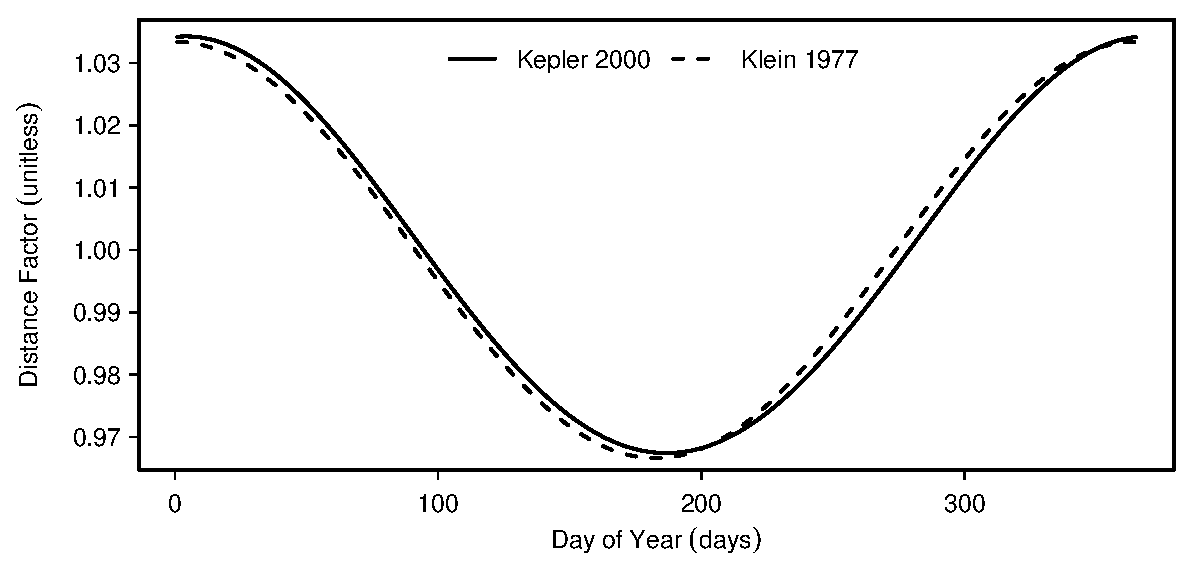
\includegraphics[width=\textwidth]{kepler_v_klein.eps}
    \caption{Comparison between actual distance factor, $d_r$, using the simplified Kepler method for 2000 CE, and the approximation method by Klein (1977).}
    \label{fig:klein}
\end{figure}

%% \\\\\\\\\\\\\\\\\\\\\\\\\\\\\\\\\\\\\\\\\\\\\\\\\\\\\\\\\\\\\\\\\\\\\\\\ %%
%% PART 2.03.3 -- INCLINATION FACTOR, unitless
%% //////////////////////////////////////////////////////////////////////// %%
\subsubsection{Inclination factor}
\label{sec:cosz}
The inclination factor, $\cos \theta_z$, attenuates the incident solar radiation perpendicular to earth's surface to account for earth's tilted surface at different latitudes. 
The sun's elevation angle above the horizon is measured by the zenith angle ($\theta_z$). 
A general expression relating the angle of incidence ($\theta$), to other angles that describe the geometric relationship between a plane on the surface of the earth and an incoming beam of solar radiation is given by \parencite[Eq. 1.6.2]{duffie13}:

%% ------------------------------------------------------------------------ %%
%% eq:theta | Angle of incidence
%% ------------------------------------------------------------------------ %%
\begin{equation}
\label{eq:theta}
    \begin{split}
    	\cos \theta = & \sin\delta\: \sin\phi\: \cos\beta \\
            & - \sin\delta\: \cos\phi\: \sin\beta\: \cos\gamma \\
            & + \cos\delta\: \cos\phi\: \cos\beta\: \cos H \\
            & + \cos\delta\: \sin\phi\: \sin\beta\: \cos\gamma\: \cos H \\
            & + \cos\delta\: \sin\beta\: \sin\gamma\: \sin H
    \end{split}
\end{equation}

\noindent where: \\
\indent $\delta$ = declination angle, radians \\
\indent $\phi$ = latitude, radians \\
\indent $\beta$ = slope, radians \\
\indent $\gamma$ = surface azimuth angle, radians \\
\indent $H$ = hour angle, radians \\

For a horizontal surface (i.e., $\beta$ = 0), the angle of incidence below the zenith (i.e., $0^{\circ} \leq \theta_z \leq 90^{\circ}$) is given by \parencite{wetherald72, duffie13, loutre03}:

%% ------------------------------------------------------------------------ %%
%% eq:thetaz | Angle of incidence on horizontal surface
%% ------------------------------------------------------------------------ %%
\begin{equation}
\label{eq:thetaz}
	\cos \theta_z = \sin\delta\: \sin\phi + 
	                \cos\delta\: \cos\phi\: \cos H
\end{equation}

For a given latitude, $\phi$, there are two terms that need to be computed for the calculation of the inclination factor: the declination angle ($\delta$) and the hour angle ($H$).

%% \\\\\\\\\\\\\\\\\\\\\\\\\\\\\\\\\\\\\\\\\\\\\\\\\\\\\\\\\\\\\\\\\\\\\\\\ %%
%% PART 2.03.4 -- DECLINATION ANGLE, radians
%% //////////////////////////////////////////////////////////////////////// %%
\subsubsection{Declination angle}
\label{sec:delta}
The declination angle is defined as the angular position between the sun at solar noon and the earth's equator (ranging from -23.45$^{\circ}$ during the winter solstice to 23.45$^{\circ}$ during the summer solstice). 
The following calculation method for $\delta$ is for any given time of year \parencite{woolf68, loutre03}:

%% ------------------------------------------------------------------------ %%
%% eq:delta | Earth's declination angle, radians
%% ------------------------------------------------------------------------ %%
\nomenclature{$\delta$}{Declination angle, radians}
\begin{equation}
\label{eq:delta}
    \delta = \arcsin\left(\sin\lambda\:\sin\epsilon\right)
\end{equation}

\noindent where: \\
\indent $\lambda$ = heliocentric longitude relative to the vernal equinox, radians\\
\indent $\epsilon$ = obliquity of earth's axis, radians\\

Obliquity, or the off-vertical axial tilt around which the earth rotates, is the third time-varying orbital parameter (the other two being $e$ and $\omega$).  
The obliquity angle varies between 22.1$^{\circ}$ and 24.5$^{\circ}$ with a periodicity of about 41000 years \parencite{hays76}. 
A value for the 2000 CE epoch is given in Table \ref{tab:constants}.

%% ------------------------------------------------------------------------ %%
%% fig:delta | Comparison of declination angles
%% ------------------------------------------------------------------------ %%
\begin{figure}[ht!]
    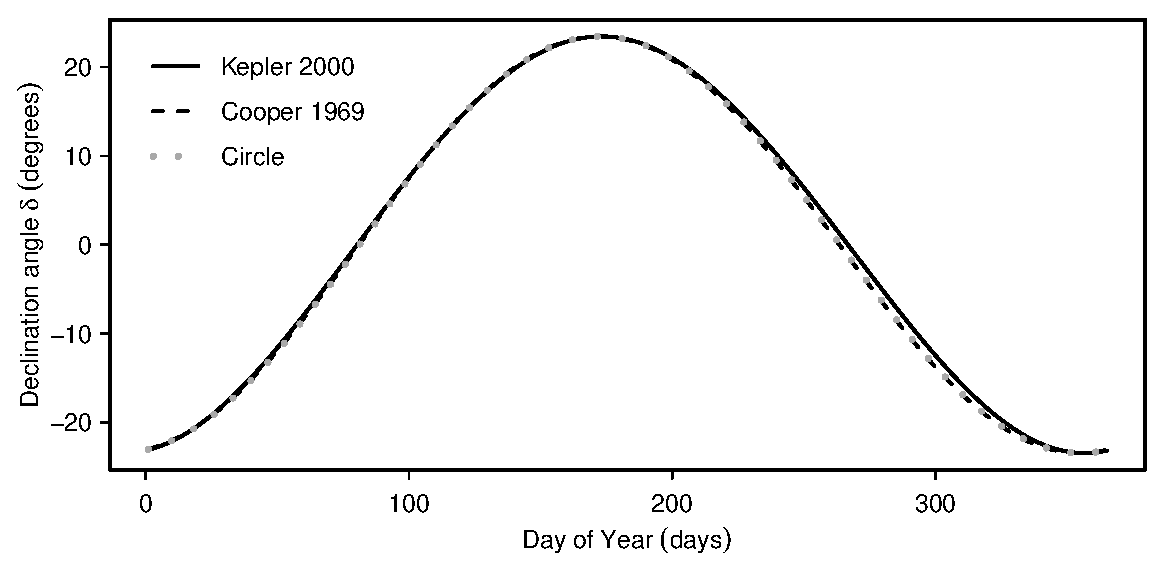
\includegraphics[width=\textwidth]{declination.eps}
    \caption{Comparison between actual declination angle, $\delta$, using the simplified Kepler method for 2000 CE, the approximation method by Cooper (1969), and the perfect circle approximation.}
    \label{fig:delta}
\end{figure}

%% ------------------------------------------------------------------------ %%
%% fig:ddiff | Comparison of declination angle differences
%% ------------------------------------------------------------------------ %%
\begin{figure}[ht!]
    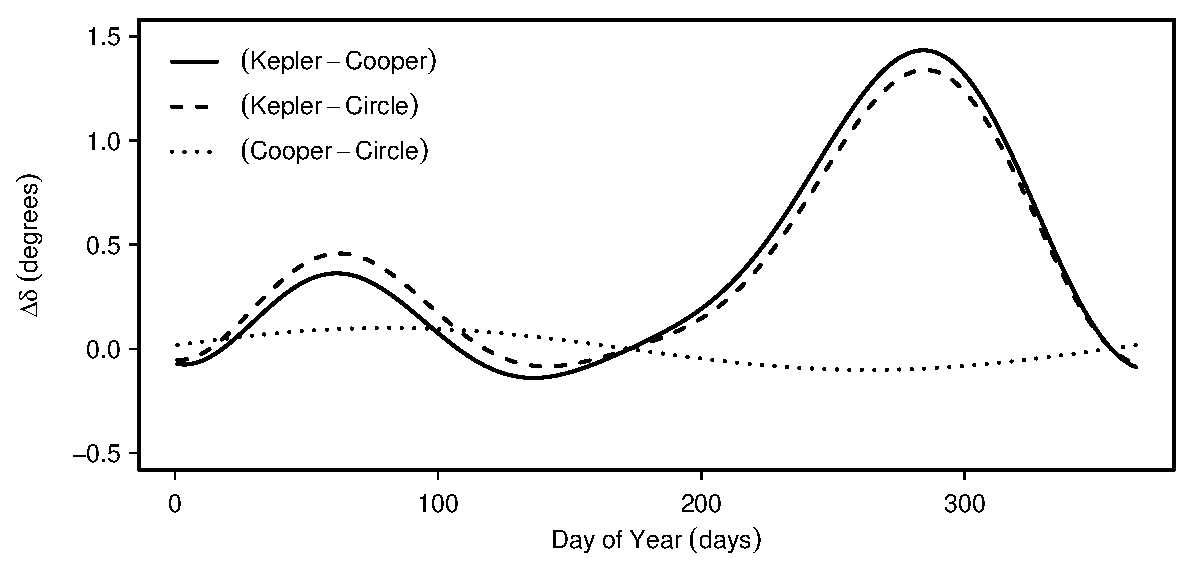
\includegraphics[width=\textwidth]{delta_difference.eps}
    \caption{Differences between actual declination angle, $\delta$, using the simplified Kepler method for 2000 CE, the approximation method by Cooper (1969), and the perfect circle approximation.}
    \label{fig:ddiff}
\end{figure}

Approximations of the declination angle have been made based on the day of the year instead of earth's longitude (similar to the distance factor approximation). 
The following assumes that earth's orbit is a perfect circle:

%% ------------------------------------------------------------------------ %%
%% eq:deltab | Declination, perfect circle approximation
%% ------------------------------------------------------------------------ %%
\begin{equation}
\label{eq:deltab}
    \delta = -\epsilon\:\cos\left(\frac{2\pi\:(n+10)}{N} \right)
\end{equation}

Another approximation includes the longitude of the perihelion \parencite{cooper69}:

%% ------------------------------------------------------------------------ %%
%% eq:deltac | Declination angle w/ longitude of perihelion
%% ------------------------------------------------------------------------ %%
\begin{equation}
\label{eq:deltac}
    \delta = \epsilon\:\sin\left(\frac{2\pi\:(n+\omega)}{N} \right)
\end{equation}

The relationship between the approximation made by Eq. \ref{eq:deltab} and Eq. \ref{eq:deltac} derives from the trigonometric identity: $-\cos x = \sin(x - \pi/2)$ and the assumption that $\omega = 283.75^{\circ}$.

\cite{spencer71} derived a third approximation to $\delta$ based on a Fourier analysis of data presented in the Nautical Almanac (1950 C.E. epoch), given in units of radians:
%% ------------------------------------------------------------------------ %%
%% eq:spencer | Declination, Spencer's method
%% ------------------------------------------------------------------------ %%
\begin{equation}
\label{eq:spencer}
\begin{split}
	\delta = & 0.006918 - 0.399912\:\cos B + 0.070257\:\sin B - \\
             & 0.006758 \:\cos 2B + 0.000907\:\sin 2B - \\
             & 0.0022697\:\cos 3B + 0.00148 \:\sin 3B
\end{split}
\end{equation} 

\noindent where $B = 2\pi\:\left(n-1\right)\: N^{-1}$.

A comparison of $\delta$ as calculated by Eq. \ref{eq:delta}, Eq. \ref{eq:deltab}, and Eq. \ref{eq:deltac} is given in Figure \ref{fig:delta}. 
There is a slight difference between the results given by Eq. \ref{eq:deltab} and Eq. \ref{eq:deltac} due to the allowance of variability in $\omega$. 
Similar to Figure \ref{fig:klein}, the largest difference between the approximation methods and that calculated by Eq. \ref{eq:delta} happens in the latter half of the year (see Figure \ref{fig:ddiff}).\\

%% \\\\\\\\\\\\\\\\\\\\\\\\\\\\\\\\\\\\\\\\\\\\\\\\\\\\\\\\\\\\\\\\\\\\\\\\ %%
%% PART 2.03.5 -- THE HOUR ANGLE, radians
%% //////////////////////////////////////////////////////////////////////// %%
\subsubsection{Hour angle}
\label{sec:hour}
The hour angle, $H$, is the angular displacement of the sun east or west of the local meridian. 
It is measured ranging from -180$^{\circ}$ to 180$^{\circ}$ with 0$^{\circ}$ occurring at solar noon. 
An approximation of the hour angle is given as follows \parencite{cooper69}:

%% ------------------------------------------------------------------------ %%
%% eq:houra | Hour angle approximation
%% ------------------------------------------------------------------------ %%
\begin{equation}
\label{eq:houra}
    H = \frac{2\pi}{24} \: (d_{s} - h_s)
\end{equation}

\noindent where: \\
\indent $d_s$ = number of daylight hours, hr \\
\indent $h_s$ = number of hours past sunrise\\

The approximation made in Eq. \ref{eq:houra} is based on the average rate of earth's spin (i.e., 360$^{\circ}$ per 24 hr). 
Knowledge of the sunrise hour is necessary for computing Eq. \ref{eq:houra}.

A more precise method of calculating $H$ follows \parencite[Eq. 3.1]{stine01}:

%% ------------------------------------------------------------------------ %%
%% eq:hour | Hour angle, radians
%% ------------------------------------------------------------------------ %%
\nomenclature{$H$}{Hour angle, radians}
\begin{equation}
\label{eq:hour}
    H = \frac{2\pi}{24} \: (t_{s} - 12)
\end{equation}

\noindent where: \\
\indent $t_{s}$ = solar time, hr \\

\noindent Solar time is the apparent angular motion of the sun across the sky with solar noon representing the time when the sun crosses the local meridian of the observer. 
The conversion between local clock time ($LCT$) and solar time ($t_{s}$) depends on the physical observation location, the day of the year, and the time zone of the location.  
The conversion equation takes the form of \parencite[Eq. 3.5]{stine01}:

%% ------------------------------------------------------------------------ %%
%% eq:soltime | Solar time, hr
%% ------------------------------------------------------------------------ %%
\nomenclature{$t_s$}{Solar time, hr}
\nomenclature{$LCT$}{Local clock time, hr}%
\nomenclature{$DS$}{Daylight savings correction factor, hr}
\begin{equation}
\label{eq:soltime}
    t_{s} = LCT + \frac{EOT}{60} - LC - DS
\end{equation}

\noindent where: \\
\indent $LCT$ = local clock time, hr \\
\indent $EOT$ = equation of time, min \\
\indent $LC$ = longitude correction factor, hr \\
\indent $DS$  = daylight savings correction factor, hr\\

\noindent The equation of time ($EOT$) is the measure of difference between the mean solar time and the true solar time.  
Due to the seasonal changes which account for the mean solar time, the actual solar time can be as great at $\pm$17 min from the mean \parencite{stine01}.  
An approximation of $EOT$ (in minutes) is given by \parencite[Eq. 1.6]{woolf68}:

%% ------------------------------------------------------------------------ %%
%% eq:eota | Equation of time, Woolf's approximation
%% ------------------------------------------------------------------------ %%
\begin{equation}
\label{eq:eota}
	\begin{split}
    	EOT = 60 \cdot ( & 0.004289 \: \cos B \\
                              & - 0.12357 \: \sin B \\
                              & - 0.060783 \: \cos 2B \\ 
                              & - 0.153809 \: \sin 2B)
	\end{split}
\end{equation}

\noindent where: \\
\indent $B = 2\pi\: (n-1)\: N^{-1}$ \\

An updated calculation of $EOT$ was developed \parencite{spencer71} and corrected \parencite{oglesby98}, accurate to within 35 seconds, and is presented in units of minutes \parencite{iqbal83}:

%% ------------------------------------------------------------------------ %%
%% eq:eotb | Equation of time, Spencer's formula
%% ------------------------------------------------------------------------ %%
\nomenclature{$EOT$}{Equation of time, min}
\begin{equation}
\label{eq:eotb}
	\begin{split}
    	EOT = \frac{1440}{2\pi} \times ( & 7.5 \times 10^{-6} \\ 
        	& + 1.868 \times 10^{-3} \: \cos B \\ 
            & - 3.2077 \times 10^{-2} \: \sin B \\
            & - 1.4615 \times 10^{-2} \: \cos 2B \\
            & - 4.0849 \times 10^{-2} \: \sin 2B)
	\end{split}
\end{equation}

\noindent where the factor $(1440)/(2\pi) \approx 229.18)$ converts radians into minutes based on the 24 hours required for the earth to make a full rotation (i.e., $2\pi$ radians). 
Figure \ref{fig:eot} shows a comparison between $EOT$ as calculated using Eq. \ref{eq:eota} and Eq. \ref{eq:eotb}. 
The difference between these two methods varies between approximately $\pm$0.45 minutes (i.e., $\pm$27 seconds).\\

%% ------------------------------------------------------------------------ %%
%% fig:eot | Comparison of EOT
%% ------------------------------------------------------------------------ %%
\begin{figure}[ht!]
    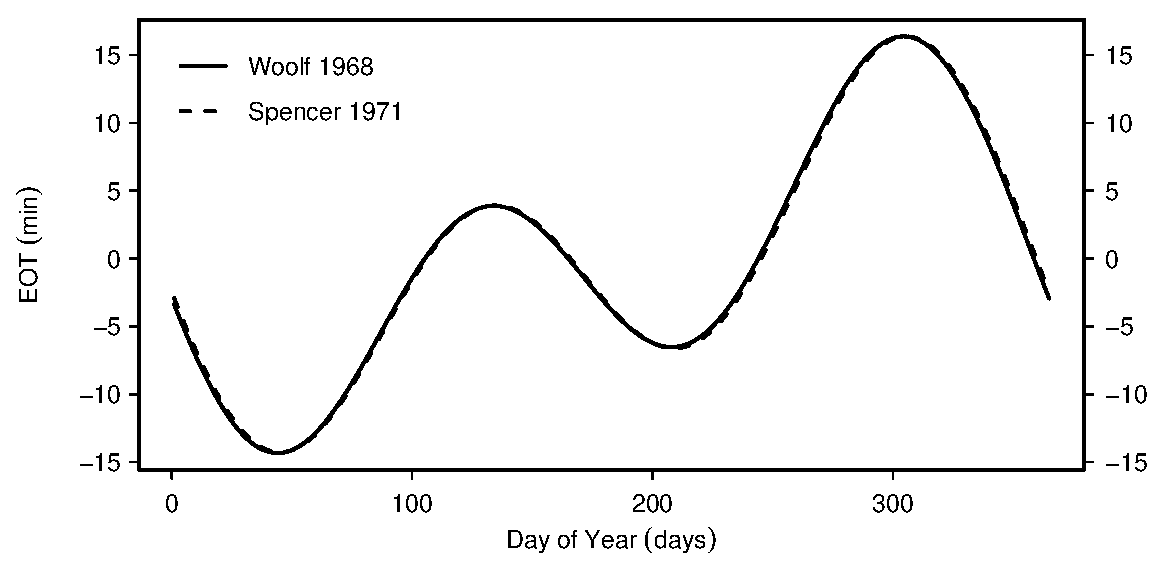
\includegraphics[width=\textwidth]{eot.eps}
    \caption{Comparison between $EOT$ as calculated by Woolf (1968) and Spencer (1971).}
    \label{fig:eot}
\end{figure}

The longitude correction factor ($LC$) makes the appropriate adjustment for the local time zone difference from the UTM/GMT based on the rotational speed of the Earth ($2\pi$ radians in 24 hours) and is given by \parencite{stine01}:

%% ------------------------------------------------------------------------ %%
%% eq:lc | Longitude correction factor, hr
%% ------------------------------------------------------------------------ %%
\nomenclature{$LC$}{Longitude correction factor, hr}%
\nomenclature{$TZ_{h}$}{Time-zone hours away from UTC, hr}%
\nomenclature{$\theta_{lon}$}{Observer's longitude, radians}
\begin{equation}
\label{eq:lc}
    LC = \left(\frac{\pi}{12}\: TZ_h - \theta_{lon}\right)\:
    \frac{12}{\pi}
\end{equation}

\noindent where: \\
\indent $TZ_{h}$ = number of time zones away from UTC, hr \\
\indent $\theta_{lon}$ = longitude of observation, radians \\

The daylight savings time correction factor, $DS$, corrects local time when summer time is in (i.e., $DS$ = 1) and is ignored otherwise.

%% \\\\\\\\\\\\\\\\\\\\\\\\\\\\\\\\\\\\\\\\\\\\\\\\\\\\\\\\\\\\\\\\\\\\\\\\ %%
%% PART 2.03.6 -- TRUE LONGITUDE, radians
%% //////////////////////////////////////////////////////////////////////// %%
\subsubsection{True longitude}
\label{sec:lambda}
Earth's true longitude, $\lambda$, (i.e., the heliocentric longitude relative to the vernal equinox) can be estimated for a given day, $n$. 
A simple estimation is given assuming a constant orbital velocity by \parencite{woolf68}:

%% ------------------------------------------------------------------------ %%
%% eq:lambda | Heliocentric longitude w.r.t. vernal equinox
%% ------------------------------------------------------------------------ %%
\nomenclature{$\lambda$}{Heliocentric longitude relative to vernal equinox, radians}
\begin{equation}
\label{eq:woolf}
	\begin{split}
    	\lambda = & 279.9348 + B \\
    	          & + 1.914827 \: \sin B - 0.079525 \: \cos B \\
    	          & + 0.019938 \: \sin 2B - 0.00162 \: \cos 2B
    \end{split}
\end{equation} 

\noindent where: \\
\indent $B = 360 \left(n - 1\right)\: N^{-1}$ \\

\noindent Note that $B$ in Eq. \ref{eq:woolf} must be units of degrees, so special attention must be given during the calculation of the sine and cosine of the angle.

\cite{berger78} presents an algorithm for computing the true longitude for a given day, $n$, based on a mean earth orbit. 
The method first computes a mean longitude, $\lambda_{m0}$, for the day of the vernal equinox (assumed 21 March, $n = 80$ for a 365-day year): 
%% ------------------------------------------------------------------------ %%
%% eq:lambdamo | Mean longitude at vernal equinox
%% ------------------------------------------------------------------------ %%
\begin{equation}
\label{eq:lambdamo}
\begin{split}
	\lambda_{m0} = & 2\left(\frac{e}{2}+\frac{e^3}{8}\right)\left(1+\beta\right)\:\sin\alpha - \\
	& \frac{e^2}{2}\left(\frac{1}{2}+\beta\right)\sin 2\alpha + \\
	& \frac{e^3}{4}\left(\frac{1}{3}+\beta\right)\:\sin 3\alpha
\end{split}
\end{equation}

\noindent where $\beta = \sqrt{1-e^2}$. 
The mean longitude for a given day, $\lambda_m$, is then calculated assuming a constant orbital speed: 
%% ------------------------------------------------------------------------ %%
%% eq:lambdam | Mean longitude
%% ------------------------------------------------------------------------ %%
\begin{equation}
\label{eq:lambdam}
	\lambda_m = \lambda_{m0} + \frac{2\pi\left(n-80\right)}{N}
\end{equation}

\noindent and the true longitude is then back-calculated from the mean longitude:
%% ------------------------------------------------------------------------ %%
%% eq:lambdat | True longitude for Berger's method
%% ------------------------------------------------------------------------ %%
\begin{equation}
\label{eq:lambdat}
	\lambda = \lambda_m + \left(2e-\frac{1}{4}e^3\right)\:\sin\nu_m + \frac{5}{4}e^2\:\sin 2\nu_m + \frac{13}{12}e^3\:\sin 3\nu_m
\end{equation}

\noindent where $\nu_m = \lambda_m - \alpha$. 

A third approximation to $\lambda$ is derived from Kepler's laws of planetary motion. 
The derivation begins with the formulaic expression of Kepler's second law of planetary motion:

\begin{quote}
	\textit{``A line joining a planet and the Sun sweeps out equal areas during equal intervals of time.''}--- Kepler's Second Law
\end{quote}

%% ------------------------------------------------------------------------ %%
%% eq:keplerb | Kepler's Second Law
%% ------------------------------------------------------------------------ %%
\begin{equation}
\label{eq:keplerb}
	\frac{dA_s}{dt} = \frac{r^2}{2} \: \frac{d\nu}{dt}
\end{equation} 

\noindent where:\\
\indent $A_s$ = sweep area of the ellipse, km$^{2}$ \\
\indent $t$ = time during which a planet has traveled some distance, days\\
\indent $\nu$ = heliocentric longitude relative to the perihelion, radians \\
\indent $r$ = distance from a planet to the sun, km \\

Integrating the left-hand side of Eq. \ref{eq:keplerb} results in the area of an ellipse, such that:

%% ------------------------------------------------------------------------ %%
%% eq:intkb | Integral of Kepler's Second Law
%% ------------------------------------------------------------------------ %%
\begin{equation}
\label{eq:intkb}
	\frac{2\pi \: a \: b}{N} = r^2\:\frac{d\nu}{dt}
\end{equation} 

\noindent where:\\
\indent $a$ = length of the semi-major axis of earth's orbit, km \\
\indent $b$ = length of the semi-minor axis of earth's orbit, km \\
\indent $N$ = earth's orbital period, days\\

To keep Eq. \ref{eq:intkb} in terms of the semi-major axis, $a$, and eccentricity, $e$, the equation for eccentricity can be solve for $b$:

%% ------------------------------------------------------------------------ %%
%% eq:b | Equation of ellipse solved for b
%% ------------------------------------------------------------------------ %%
\begin{equation}
\label{eq:b}
	b = a \: \sqrt{1 - e^2}
\end{equation} 

The angular velocity, $d\nu/dt$, can now be solved by replacing Eq. \ref{eq:b} into Eq. \ref{eq:intkb}:

%% ------------------------------------------------------------------------ %%
%% eq:nudota | Equation for orbital velocity
%% ------------------------------------------------------------------------ %%
\begin{equation}
\label{eq:nudota}
	\frac{d\nu}{dt} = \left(\frac{a}{r}\right)^2\:\frac{2\pi\sqrt{1-e^2}}{N}
\end{equation} 

Substituting Eq. \ref{eq:r} into Eq. \ref{eq:nudota} yields:

%% ------------------------------------------------------------------------ %%
%% eq:nudotb | Equation for orbital velocity
%% ------------------------------------------------------------------------ %%
\begin{equation}
\label{eq:nudotb}
	\frac{d\nu}{dt} = \frac{2\pi}{N}\:\frac{\left(1+e\:\cos\nu\right)^2}
	                                      {\left(1-e^2\right)^{1.5}}
\end{equation} 

A methodology for solving the heliocentric longitude for a given time, $t$, follows \parencite{kutzbach88}:

%% ------------------------------------------------------------------------ %%
%% eq:dtdnu | Equation for dt given dnu
%% ------------------------------------------------------------------------ %%
\begin{equation}
\label{eq:dtdnu}
	dt = \frac{N\:\left(1-e^2\right)^{1.5}}{2\pi}\:\left(1+e\:\cos\nu\right)^{-2} d\nu
\end{equation}

\noindent Integrating both sides results in:

%% ------------------------------------------------------------------------ %%
%% eq:tdnu | Equation for t given dnu, days
%% ------------------------------------------------------------------------ %%
\begin{equation}
\label{eq:tdnu}
	t = \frac{N\:\left(1-e^2\right)^{1.5}}
	         {2\pi}\:\int\left(1+e\:\cos\nu\right)^{-2} d\nu
\end{equation}

The non-trivial integrand on the right-hand side of Eq. \ref{eq:tdnu} has a long and complicated integral, which was solved using the Maxima computer algebra system\footnotemark \footnotetext{\url{http://maxima.sourceforge.net/}}. 

%% ------------------------------------------------------------------------ %%
%% eq:dnu | Integral of dnu
%% ------------------------------------------------------------------------ %%
\begin{equation}
\label{eq:dnu}
	\begin{split}
		\int & \left(1+e\:\cos\nu\right)^{-2} d\nu = \\ 
			& 2\:\frac{\arctan \left( 
				\frac{(2e-2)\:\sin\nu}{2\sqrt{1-e^2}\:(\cos\nu +1)}
			    \right)}
			             {\sqrt{1-e^2}\:(e^2-1)} + \\
			& -2 \:\frac{e\:\sin\nu}
			    {(\cos\nu +1) \:\left(  
			    	\frac{(e^3-e^2-e+1)\:\sin^2\nu}{(\cos\nu +1)^2}
			    	- e^3 -e^2 + e + 1
			    \right) }
	\end{split}
\end{equation}

An approximation to this integral can be made assuming that eccentricity is small, such that higher powers of eccentricity can be ignored. 
Following the elimination of high-powered eccentricity terms:

%% ------------------------------------------------------------------------ %%
%% eq:dnusimpa | Simplification (a) to integral of dnu
%% ------------------------------------------------------------------------ %%
\begin{equation}
\label{eq:dnusimpa}
	\begin{split}
		\int & \left(1+e\:\cos\nu\right)^{-2} d\nu \approx \\ 
			& -2\:\arctan \left( 
				\frac{(e-1)\:\sin\nu}{\cos\nu +1}
			    \right) + \\
			& -2\:\frac{e\:\sin\nu\:(\cos\nu +1)}
			    {(1-e)\:\sin^2\nu + (1+e)\:(\cos\nu +1)^2}
	\end{split}
\end{equation}

\noindent Now, assume that eccentricity in the quantities $(e-1)$, $(1-e)$, and $(1+e)$ is negligible.

%% ------------------------------------------------------------------------ %%
%% eq:dnusimpb | Simplification (b) to integral of dnu
%% ------------------------------------------------------------------------ %%
\begin{equation}
\label{eq:dnusimpb}
	\begin{split}
		\int & \left(1+e\:\cos\nu\right)^{-2} d\nu \approx \\ 
			& 2\:\arctan \left( 
				\frac{\sin\nu}{\cos\nu +1}
			    \right) - \frac{2e\:\sin\nu\:(\cos\nu +1)}
			    {\sin^2\nu + \cos^2\nu + 2\cos\nu + 1}
	\end{split}
\end{equation}

\noindent Finally, simplifying the second term leads to:

%% ------------------------------------------------------------------------ %%
%% eq:dnusimpc | Simplification (c) to integral of dnu
%% ------------------------------------------------------------------------ %%
\begin{equation}
\label{eq:dnusimpc}
		\int \left(1+e\:\cos\nu\right)^{-2} d\nu \approx 
			2\:\arctan \left( \frac{\sin\nu}{\cos\nu +1}
			\right) - e\:\sin\nu
\end{equation}

%% ------------------------------------------------------------------------ %%
%% fig:dkepler | Difference betweeen full and simplified Kepler methods
%% ------------------------------------------------------------------------ %%
\begin{figure}[ht!]
    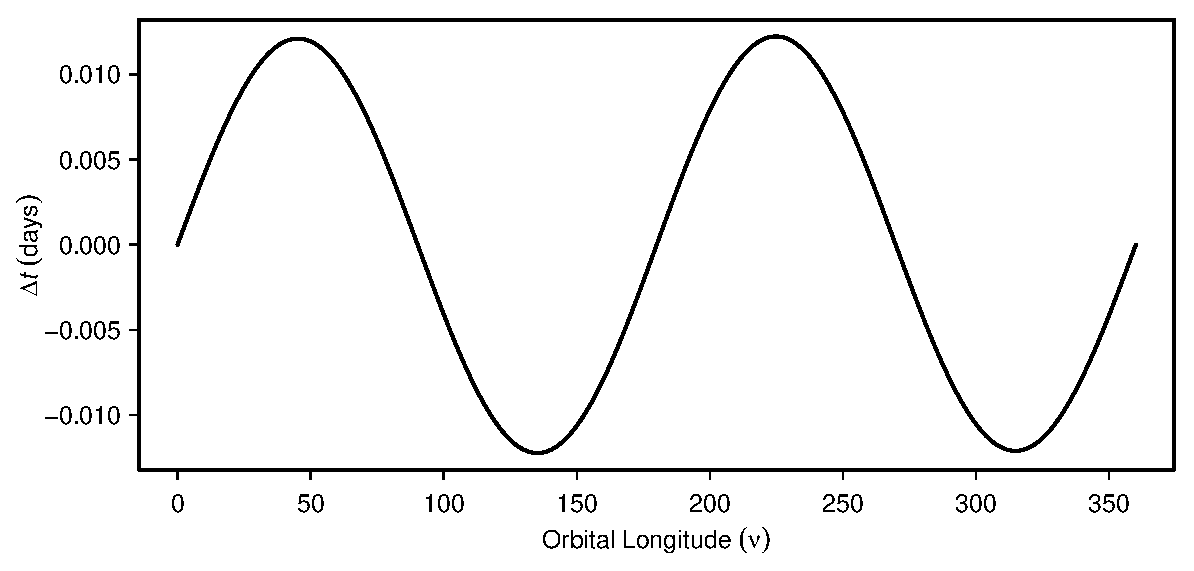
\includegraphics[width=\textwidth]{kepler_diff.eps}
    \caption{Difference between the full integral and simplified integral solutions of $t$ for a given $\nu$.}
    \label{fig:dkepler}
\end{figure}

\noindent A comparison between the full derivative (i.e., Eq. \ref{eq:dnu}) and the simplification (i.e., Eq. \ref{eq:dnusimpc}) revealed a discrepancy in the magnitude of the second term in Eq. \ref{eq:dnusimpc} by a factor of two. 
Following this addition, substituting it back into Eq. \ref{eq:tdnu}, and assuming that $(1-e^2)^{1.5} \approx 1$, the equation for the simplified Kepler mapping is:

%% ------------------------------------------------------------------------ %%
%% eq:tnu | Equation for t given nu, days
%% ------------------------------------------------------------------------ %%
\begin{equation}
\label{eq:tnu}
	t = \frac{N}{\pi}\:\left( \arctan \left( \frac{\sin\nu}{\cos\nu + 1} \right) - e \:\sin\nu \right)
\end{equation}

Figure \ref{fig:dkepler} shows the difference between Eq. \ref{eq:tdnu} and Eq. \ref{eq:tnu} (full integral versus the simplified integral). 
The magnitude of the difference between the two methods is approximately 35.2 minutes, which is more than reasonable given the amount of simplification that was made.

To complete the mapping, the calendar days of a particular year need to be associated with $t$ in Eq. \ref{eq:tnu}. 
This is accomplished through the definition of $\lambda$ (i.e., Eq. \ref{eq:nu}). 
For a known $\omega$, $\nu$ at the vernal equinox can be solved by setting $\lambda = 0$. 
First find the number of days it takes the earth to travel from the perihelion ($\nu = 0$) to the vernal equinox ($\nu(\text{V.E.}) = 360-\omega$) by solving Eq. \ref{eq:tnu}. 
Next, either solve for specific day of the year, $n$, on which the vernal equinox falls (i.e., Appendix \ref{app:equinox}) or assume a constant day of the year (e.g., $n(\text{V.E.}) = 80$). 
The difference between $n(\text{V.E.})$ and $t(\nu(\text{V.E.}))$ corresponds to the calendar day at the perihelion.

For example, assuming the current value of $\omega = 283^{\circ}$, then $t(360-\omega) = 76.2$ days. 
The difference between a constant $n(\text{V.E.}) = 80$ and $t$ at the vernal equinox is 3.8 days. 
This is reasonable given that the date of the perihelion is typically within the first week of January. 

In order to get $\lambda$ for a given $n$, solve Eq. \ref{eq:tnu} for each 1$^{\circ}$ of $\nu$. 
Next, find the value of $t$ that is as close to, but not greater than $n$.   
Then, move the earth forward in space equivalent to the orbital velocity at position $\nu(t)$ multiplied by the difference in time (i.e., $n-t$) using Eq. \ref{eq:nudotb}. 
Lastly, use Eq. \ref{eq:nu} to solve for $\lambda(n)$, making certain to keep values of $\lambda \leq 360^{\circ}$.

%% \\\\\\\\\\\\\\\\\\\\\\\\\\\\\\\\\\\\\\\\\\\\\\\\\\\\\\\\\\\\\\\\\\\\\\\\ %%
%% PART 2.04 -- DAILY ET SOLAR RADIATION, J/m^2
%% //////////////////////////////////////////////////////////////////////// %%
\subsection{Daily Extraterrestrial Solar Radiation}
\label{sec:dra}
Often, it is necessary to calculate the total daily solar irradiance (i.e., the integration of instantaneous solar irradiance over the course of the day). 
This can be analytically done by integrating the instantaneous extraterrestrial solar radiation curve, defined by Eq. \ref{eq:etsr} (see \S \ref{sec:ra}), over the daylight hours. 

Using the definition of the hour angle, $H$ (see \S \ref{sec:hour}), the sunset angle, $H_s$, can be calculated when $R_a = 0$. 
Using the inclination factor for horizontal surfaces (i.e., Eq. \ref{eq:thetaz}) the equation for instantaneous solar radiation is:

%% ------------------------------------------------------------------------ %%
%% eq:irah | Instantaneous solar radiation on horizontal surface, W/m^2
%% ------------------------------------------------------------------------ %%
\begin{equation}
\label{eq:irah}
	R_a = G_{sc}\: d_r\: \left( \sin\delta\: \sin\phi + 
	      \cos\delta\: \cos\phi\: \cos H \right)
\end{equation}

\noindent Setting Eq. \ref{eq:irah} equal to zero and solving for the sunset hour angle:

%% ------------------------------------------------------------------------ %%
%% eq:hs | Sunset hour angle, radians
%% ------------------------------------------------------------------------ %%
\begin{equation}
\nomenclature{$H_s$}{Sunset hour angle, radians}
\label{eq:hs}
	H_s  = \arccos\left(\frac{-\sin\delta\: \sin\phi}
		                          {\cos\delta\: \cos\phi}\right)
		 = \arccos\left(-\tan\delta\: \tan\phi\right)
\end{equation}

\noindent where:\\
\indent $H_s$ = sunset hour angle, radians\\
\indent $\delta$ = declination angle, radians\\
\indent $\phi$ = latitude, radians\\

\noindent Special care needs to be made when $\tan\delta\:\tan\phi \geq 1$ (i.e., polar day, no sunset, $H_s = \pi$) and when $\tan\delta\:\tan\phi \leq -1$ (i.e., polar night, no sunrise, $H_s = 0$).

The daylight hours are calculated from sunrise, $-H_s$, to sunset, $H_s$. 
To calculate the daylight hours, $d_s$, double the sunset hour (to accommodate for the time between sunrise and solar noon) and convert the angle to hours, based on the rate of earth's rotation (i.e., 24 hours per $2\pi$ radians):

%% ------------------------------------------------------------------------ %%
%% eq:ds | Daylight hours, hr
%% ------------------------------------------------------------------------ %%
\nomenclature{$d_s$}{Hours of daylight, hr}
\begin{equation}
\label{eq:ds}
	d_s  = \frac{24\: H_s}{\pi}
\end{equation}

\noindent where:\\
\indent $d_s$ = hours of daylight, hr\\
\indent $H_s$ = sunset hour angle, radians \\ 

The daily integral of solar radiation can now be solved by integrating Eq. \ref{eq:irah} from solar noon, $H_o$, to sunset, $H_s$ (see Figure \ref{fig:intra}):

%% ------------------------------------------------------------------------ %%
%% fig:intra | Half-day integral of Ra
%% ------------------------------------------------------------------------ %%
\begin{figure}[ht!]
    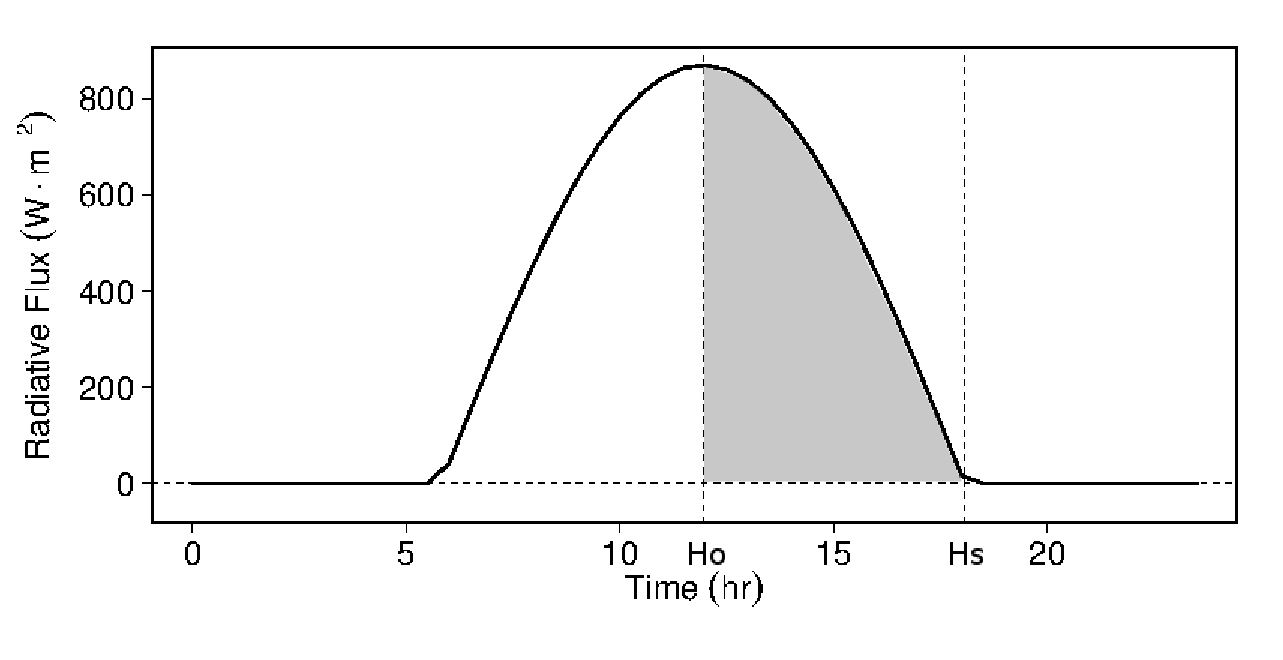
\includegraphics[width=\textwidth]{int_ra.eps}
    \caption{Half-day integral of $R_a$ from solar noon, $H_o$, to sunset, $H_s$ (shaded area).}
    \label{fig:intra}
\end{figure}

%% ------------------------------------------------------------------------ %%
%% eq:intrahs | Integral of Ra from solar noon to Hs
%% ------------------------------------------------------------------------ %%
\begin{equation}
\label{eq:intrahs}
	\int_0^{H_s} R_a = G_{sc}\: d_r\: \left( 
	      \sin\delta\: \sin\phi\: H_s + 
	      \cos\delta\: \cos\phi\: \sin H_s \right)
\end{equation}

\noindent The total daily solar radiation, $R_{Da}$, is found by doubling the quantity in Eq. \ref{eq:intrahs} (again to account for the morning half of the daily radiation curve) and converting the units integrated over from radians to seconds (i.e., 86400 seconds per day):

%% ------------------------------------------------------------------------ %%
%% eq:dayra | Daily Ra, J/m^2
%% ------------------------------------------------------------------------ %%
\nomenclature{$R_{Da}$}{Daily total extraterrestrial solar radiation, J$\cdot$m$^{-2}$}
\begin{equation}
\label{eq:dayra}
	R_{Da} = \frac{86400}{\pi}\: G_{sc}\: d_r\: \left( 
	      \sin\delta\: \sin\phi\: H_s + 
	      \cos\delta\: \cos\phi\: \sin H_s \right)
\end{equation}

\noindent where: \\
\indent $R_{Da}$ = daily total extraterrestrial solar radiation, J$\cdot$m$^{-2}$\\

%% \\\\\\\\\\\\\\\\\\\\\\\\\\\\\\\\\\\\\\\\\\\\\\\\\\\\\\\\\\\\\\\\\\\\\\\\ %%
%% PART 2.05 -- NET RADIATION FLUX, W/m^2
%%///////////////////////////////////////////////////////////////////////// %%
\subsection{Net Radiation Flux}
\label{sec:rn}
The net radiation is defined as \parencite[Eq. 4]{linacre68}:

%% ------------------------------------------------------------------------ %%
%% eq:rn | Net radiation, W/m^2
%% ------------------------------------------------------------------------ %%
\nomenclature{$R_n$}{Net radiation flux, W$\cdot$m$^{-2}$}
\begin{equation}
\label{eq:rn}
	R_n = R_{ns} - R_{nl}
\end{equation}

\noindent where: \\
\indent $R_n$ = net radiation, W$\cdot$m$^{-2}$ \\
\indent $R_{ns}$ = net shortwave downwelling solar radiation, W$\cdot$m$^{-2}$ \\
\indent $R_{nl}$ = net longwave radiation, W$\cdot$m$^{-2}$ \\

\noindent Due to the lack of observations of radiation quantities on the global scale, net shortwave and longwave radiation must be modeled.

%% \\\\\\\\\\\\\\\\\\\\\\\\\\\\\\\\\\\\\\\\\\\\\\\\\\\\\\\\\\\\\\\\\\\\\\\\ %%
%% PART 2.05.1 -- SHORTWAVE RADIATION FLUX, W/m^2
%%///////////////////////////////////////////////////////////////////////// %%
\subsubsection{Shortwave radiation flux}
\label{sec:rs}
Net incoming shortwave solar radiation, $R_{ns}$, can be modeled after the extraterrestrial solar radiation, $R_a$ (see \S \ref{sec:ra} by accounting for the amount of radiation that is reflected:

%% ------------------------------------------------------------------------ %%
%% eq:rns | Net shortwave radiation, W/m^2
%% ------------------------------------------------------------------------ %%
\nomenclature{$R_{ns}$}{Net shortwave solar radiation flux, W$\cdot$m$^{-2}$}
\begin{equation}
\label{eq:rns}
	R_{ns} = \left(1 - \beta_{sw}\right)\: R_s
\end{equation}

\noindent where: \\
\indent $R_{ns}$ = net shorwave solar radiation flux, W$\cdot$m$^{-2}$ \\
\indent $R_s$ = incident shortwave solar radiation flux, W$\cdot$m$^{-2}$ \\
\indent $\beta_{sw}$ = shortwave albedo, unitless \\

\noindent A value for the shortwave albedo, $\beta_{sw}$, is given in Table \ref{tab:constants}. 
The incident shortwave solar radiation can be expressed as the atmospheric transmittivity, $\tau$, multiplied by $R_a$:

%% ------------------------------------------------------------------------ %%
%% eq:rs | Incident shortwave radiation, W/m^2
%% ------------------------------------------------------------------------ %%
\nomenclature{$R_s$}{Incident shortwave solar radiation flux, W$\cdot$m$^{-2}$}
\begin{equation}
\label{eq:rs}
	R_s = \tau\: R_a
\end{equation}

\noindent where: \\
\indent $R_s$ = incident shortwave solar radiation flux, W$\cdot$m$^{-2}$ \\
\indent $R_a$ = extraterrestrial solar radiation flux, W$\cdot$m$^{-2}$ \\
\indent $\tau$ = atmospheric transmittivity, unitless \\

Atmospheric transmittivity may be modeled as a function of sunshine hours and elevation. 
The presence of clouds (i.e., fewer sunshine hours) reduces the amount of shortwave radiation that reaches the surface. 
Similarly, at higher elevations, there is less atmosphere through which the shortwave radiation must travel, thereby increasing the amount of radiation reaching the surface. 
Assuming a mean sea-level transmittivity level follows the \r{A}ngstrom-Prescott model:

%% ------------------------------------------------------------------------ %%
%% eq:tauo | Mean sea-level transmittivity, unitless
%% ------------------------------------------------------------------------ %%
\nomenclature{$\tau_o$}{Mean sea-level transmittivity, unitless}
\begin{equation}
\label{eq:tauo}
	\tau_o = c + d\: S_f 
\end{equation}

\noindent where: \\
\indent $\tau_o$ = mean sea-level transmittivity, unitless \\
\indent $c$ = minimum transmittivity for cloudy skies, unitless \\
\indent $d$ = angular coefficient of transmittivity, unitless \\
\indent $S_f$ = fraction of daily bright sunshine hours ($0\leq S_f\leq 1$) \\

\noindent Empirical values for $c$ and $d$ are given in Table \ref{tab:constants}. 
To accommodate the increase in transmittivity with elevation, $\tau_o$ can be corrected with a based on the regression of Beer's radiation extinction function below 3000 m with an average sun angle of 45$^{\circ}$ \parencite{allen96}:

%% ------------------------------------------------------------------------ %%
%% eq:tau | Atmospheric transmittivity, unitless
%% ------------------------------------------------------------------------ %%
\nomenclature{$\tau$}{Atmospheric transmittivity, unitless}
\begin{equation}
\label{eq:tau}
	\tau = \tau_o\:\left( 1+2.67\times 10^{-5}\: z \right)
\end{equation}

\noindent where: \\
\indent $\tau$ = elevation-corrected atmospheric transmittivity, unitless \\
\indent $z$ = elevation, m \\

%% \\\\\\\\\\\\\\\\\\\\\\\\\\\\\\\\\\\\\\\\\\\\\\\\\\\\\\\\\\\\\\\\\\\\\\\\ %%
%% PART 2.05.2 -- LONGWAVE RADIATION FLUX, W/m^2
%%///////////////////////////////////////////////////////////////////////// %%
\subsubsection{Longwave radiation flux}
\label{sec:rl}
The net outgoing longwave radiation (i.e., thermal radiation) is comprised of the difference between the surface (upward) and the atmospheric (downward) radiant heat multiplied by a cloudiness adjustment factor, which can be approximated based on mean daily air temperature \parencite{linacre68}:

%% ------------------------------------------------------------------------ %%
%% eq:rnl | Net longwave radiation, W/m^2
%% ------------------------------------------------------------------------ %%
\nomenclature{$R_{nl}$}{Net longwave radiation flux, W$\cdot$m$^{-2}$}
\begin{equation}
\label{eq:rnl}
	\begin{split}
		R_{nl} & = \left(R_{lu} - R_{ld} \right) 
		         \left(b + (1-b)\: S_f \right) \\
		       & \approx \left(b + (1-b)\: S_f \right) 
		         \left(A - T_c \right)
	\end{split}
\end{equation}

\noindent where: \\
\indent $R_{nl}$ = net longwave radiation, W$\cdot$m$^{-2}$ \\
\indent $R_{lu}$ = longwave upward radiation flux, W$\cdot$m$^{-2}$\\
\indent $R_{ld}$ = longwave clear-sky downward radiation flux, W$\cdot$m$^{-2}$\\
\indent $b$ = empirical constant\\
\indent $S_f$ = fraction of daily bright sunshine hours \\
\indent $A$ = empirical constant \\
\indent $T_c$ = mean daily air temperature, $^{\circ}$C \\

\noindent Values for $A$ and $b$ are given in Table \ref{tab:constants}. 
The upward flux of longwave radiation may be modeled assuming a constant emissivity (e.g., under well-watered conditions) \parencite[Eq. 21]{linacre68}:

%% ------------------------------------------------------------------------ %%
%% eq:rlu | Longwave upward radiation, W/m^2
%% ------------------------------------------------------------------------ %%
\nomenclature{$R_{lu}$}{Longwave upward radiation flux, W$\cdot$m$^{-2}$}
\begin{equation}
\label{eq:rlu}
	R_{lu} = \sigma_{sb}\: T_k^4
\end{equation}

\noindent where: \\
\indent $R_{lu}$ = longwave upward radiation flux, W$\cdot$m$^{-2}$\\
\indent $\sigma_{sb}$ = Stefan-Boltzman constant, W$\cdot$m$^{-2}\cdot$K$^{-4}$\\
\indent $T_k$ = mean daily air temperature, K\\

\noindent The downward clear-sky atmospheric longwave radiation is given by \parencite[Eq. 20]{linacre68}:

%% ------------------------------------------------------------------------ %%
%% eq:rld | Longwave downward radiation, W/m^2
%% ------------------------------------------------------------------------ %%
\nomenclature{$R_{ld}$}{Longwave clear-sky downward radiation flux, W$\cdot$m$^{-2}$}
\begin{equation}
\label{eq:rld}
	R_{ld} = 1.19\:\sigma_{sb}\: T_k^4 - 171
\end{equation}

\noindent where: \\
\indent $R_{ld}$ = longwave clear-sky downward radiation flux, W$\cdot$m$^{-2}$\\
\indent $\sigma_{sb}$ = Stefan-Boltzman constant, W$\cdot$m$^{-2}\cdot$K$^{-4}$\\
\indent $T_k$ = mean daily air temperature, K\\

%% \\\\\\\\\\\\\\\\\\\\\\\\\\\\\\\\\\\\\\\\\\\\\\\\\\\\\\\\\\\\\\\\\\\\\\\\ %%
%% PART 2.06 -- DAILY DAYTIME NET RADIATION, J/m^2
%%///////////////////////////////////////////////////////////////////////// %%
\subsection{Daily Daytime Net Radiation}
\label{sec:drn}
The daily integration of the net radiation curve requires the definition of the cross-over hour angle when $R_n = 0$, i.e., $H_n$. 
From Eq. \ref{eq:rn}, substituting Eq. \ref{eq:rns} and Eq. \ref{eq:rs} for the shortwave radiation flux and assuming $R_a$ for a horizontal surface:

%% ------------------------------------------------------------------------ %%
%% eq:rnhn | Net radiation long equation, W/m^2
%% ------------------------------------------------------------------------ %%
\begin{equation}
\label{eq:rnhn}
	R_{n} = \left(1-\beta_{sw}\right)\:\tau\: G_{sc}\: d_r\: \left(
	        \sin\delta\: \sin\phi + 
	        \cos\delta\: \cos\phi\: \cos H
	        \right) - R_{nl}
\end{equation}

\noindent Setting $R_n = 0$ and solving Eq. \ref{eq:rnhn} for the hour angle:

%% ------------------------------------------------------------------------ %%
%% eq:hn | Net radiation cross-over hour angle, radians
%% ------------------------------------------------------------------------ %%
\begin{equation}
\label{eq:hn}
	H_{n} = \arccos \left( 
	        \frac{R_{nl}}{\left(1-\beta_{sw}\right)\:\tau\: G_{sc}\: d_r\: 
	        \cos\delta\: \cos\phi} - 
	        \tan\delta\: \tan\phi
	        \right)
\end{equation}

\noindent Eq. \ref{eq:hn} may be simplified by making the following substitutions: $r_u = \sin\delta\:\sin\phi$, $r_v = \cos\delta\:\cos\phi$, $r_w = \left(1-\beta_{sw}\right)\:\tau\: G_{sc}\: d_r$, such that Eq. \ref{eq:hn} may be rewritten as:

%% ------------------------------------------------------------------------ %%
%% eq:hns | Simple et radiation cross-over hour angle, radians
%% ------------------------------------------------------------------------ %%
\nomenclature{$H_n$}{Net radiation flux cross-over hour angle, radians}
\begin{equation}
\label{eq:hns}
	H_{n} = \arccos \left( 
	        \frac{R_{nl} - r_w\: r_u}{r_w\: r_v} 
	        \right)
\end{equation}

\noindent where:\\
\indent $H_n$ = net radiation flux cross-over hour angle, radians\\
\indent $R_{nl}$ = net longwave radiation flux, W$\cdot$m$^{-2}$\\
\indent $r_u = \sin\delta\: \sin\phi$, unitless \\
\indent $r_v = \cos\delta\: \cos\phi$, unitless \\
\indent $r_w = \left(1-\beta_{sw}\right)\:\tau\: G_{sc}\: d_r$, W$\cdot$m$^{-2}$\\

\noindent Special care needs to be made when $(R_{nl}-r_w\: r_u)/(r_w\: r_v) \geq 1$ (i.e., net radiation always less than zero, $H_n = 0$) and when $(R_{nl}-r_w\: r_u)/(r_w\: r_v) \leq -1$ (i.e., net radiation always greater than zero, $H_n = \pi$). 

The half-day integral of net radiation can now be solved by integrating Eq. \ref{eq:rnhn} from solar noon to $H_n$ (see Figure \ref{fig:intrn}):

%% ------------------------------------------------------------------------ %%
%% fig:intrn | Half-day integral of Rn
%% ------------------------------------------------------------------------ %%
\begin{figure}[ht!]
    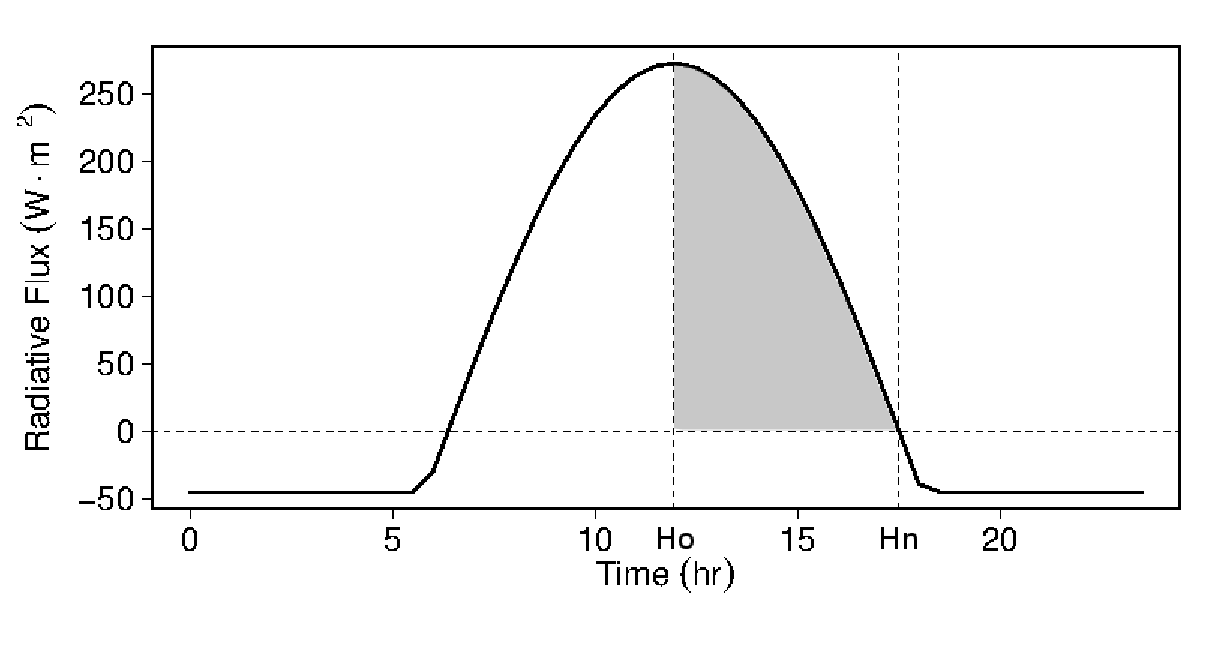
\includegraphics[width=\textwidth]{int_rn.eps}
    \caption{Half-day integral of $R_n$ from solar noon, $H_o$, to cross-over hour angle, $H_n$ (shaded area).}
    \label{fig:intrn}
\end{figure}

%% ------------------------------------------------------------------------ %%
%% eq:irnhn | Integral of net radiation
%% ------------------------------------------------------------------------ %%
\begin{equation}
\label{eq:irnhn}
	\int_0^{H_n} R_{n} = r_w\: \left(r_u\: H_n + r_v\: \sin H_n \right) - 
	R_{nl}\: H_n
\end{equation}

\noindent The total daily net radiation, $R_{Dn}$, is found by doubling the quantity in Eq. \ref{eq:irnhn} (i.e., twice the half-day amount) and converting the units integrated over from radians to seconds:

%% ------------------------------------------------------------------------ %%
%% eq:dayrn | Daily daytime net radiation, J/m^2
%% ------------------------------------------------------------------------ %%
\nomenclature{$R_{Dn}$}{Daily daytime net radiation, J$\cdot$m$^{-2}$}
\begin{equation}
\label{eq:dayrn}
	R_{Dn} = \frac{86400}{\pi}\: \left( 
	             \left( r_w\: r_u - R_{nl}\right)\: H_n + 
	             r_w\: r_v\: \sin H_n
	         \right)
\end{equation}

\noindent where: \\
\indent $R_{Dn}$ = daily daytime net radiation, J$\cdot$m$^{-2}$ \\
\indent $R_{nl}$ = net longwave radiation flux, W$\cdot$m$^{-2}$\\
\indent $H_n$ = net radiation flux cross-over hour angle, radians\\
\indent $r_u = \sin\delta\: \sin\phi$, unitless \\
\indent $r_v = \cos\delta\: \cos\phi$, unitless \\
\indent $r_w = \left(1-\beta_{sw}\right)\:\tau\: G_{sc}\: d_r$, W$\cdot$m$^{-2}$\\

%% \\\\\\\\\\\\\\\\\\\\\\\\\\\\\\\\\\\\\\\\\\\\\\\\\\\\\\\\\\\\\\\\\\\\\\\\ %%
%% PART 2.07 -- DAILY NIGHTTIME NET RADIATION, J/m^2
%%///////////////////////////////////////////////////////////////////////// %%
\subsection{Daily Nighttime Net Radiation}
\label{sec:drnn}
Some quantities, such as condensation, occur during the nighttime hours and may be modeled as a function of total nighttime net radiation. 
By utilizing the same methodology used for daily extraterrestrial solar radiation (\S \ref{sec:dra}) and daily net radiation (\S \ref{sec:drn}), total nighttime net radiation may be calculated as twice the half-day integral.

The half-day integral for the nighttime net radiation consists of two parts: the $R_n$ curve from $H_n$ to $H_s$ and the $R_{nl}$ curve from $H_s$ to solar midnight, $H_p$ (see Figure \ref{fig:intrnn}).

%% ------------------------------------------------------------------------ %%
%% fig:intrnn | Half-day integral of Rnn
%% ------------------------------------------------------------------------ %%
\begin{figure}[ht!]
    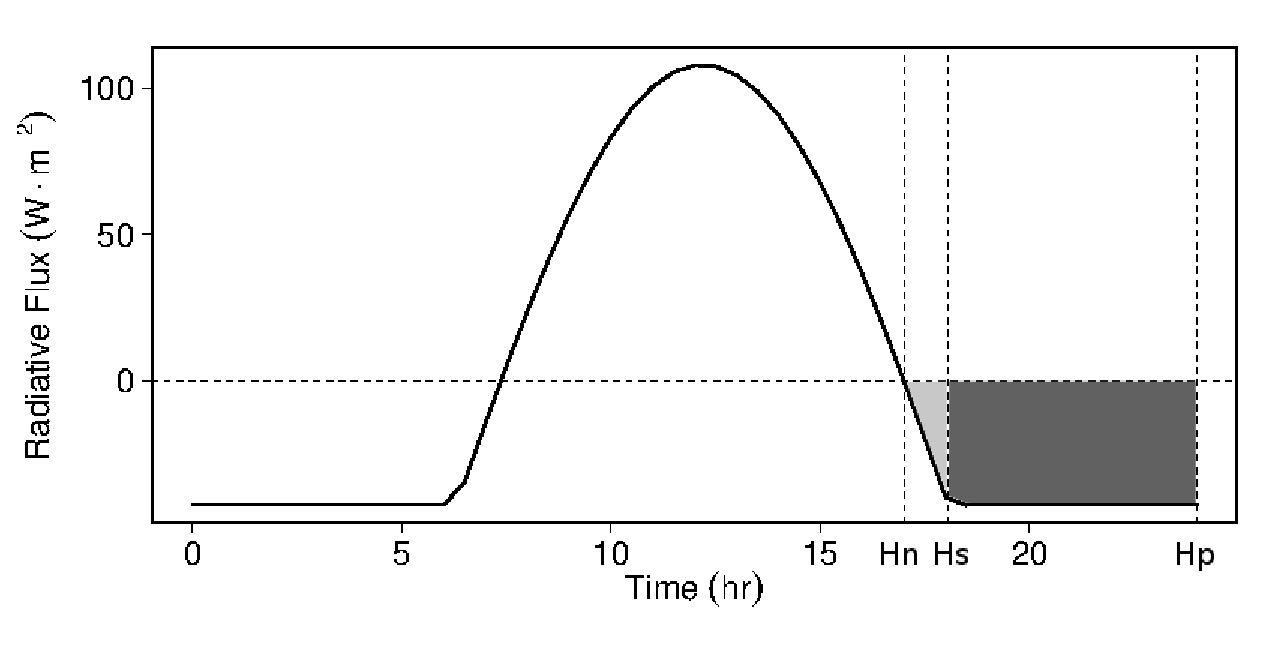
\includegraphics[width=\textwidth]{int_rnn.eps}
    \caption{Half-day integral of $R_{nn}$ from the cross-over hour, $H_n$, to sunset, $H_s$ (light shaded area) and from sunset to solar midnight, $H_p$ (dark shaded area).}
    \label{fig:intrnn}
\end{figure}

%% ------------------------------------------------------------------------ %%
%% eq:irnn | Integral of nightly net radiation relationship
%% ------------------------------------------------------------------------ %%
\begin{equation}
\label{eq:irnn}
	\int_{H_n}^{H_p} R_{n} = \int_{H_n}^{H_s} R_n + \int_{H_s}^{\pi} R_{nl}
\end{equation}

\noindent Integrating Eq. \ref{eq:irnn} and using the same variable substitutions described in \S \ref{sec:drn}:

%% ------------------------------------------------------------------------ %%
%% eq:intrnn | Integral of nightly net radiation
%% ------------------------------------------------------------------------ %%
\begin{equation}
\label{eq:intrnn}
	\begin{split}
		\int_{H_n}^{H_p} R_{n} = & r_w\: \left( r_u\: (H_s-H_n) + 
		r_v\: (\sin H_s - \sin H_n) \right) \\
		& + \left(\pi- 2\: H_s + H_n \right)\: R_{nl} 
	\end{split}
\end{equation}

\noindent The total nightly net radiation, $R_{Dnn}$ is found by doubling the integral of Eq. \ref{eq:irnn} and converting the units integrated over from radians to seconds:

%% ------------------------------------------------------------------------ %%
%% eq:irnn | Integral of nightly net radiation relationship, J/m^2
%% ------------------------------------------------------------------------ %%
\nomenclature{$R_{Dnn}$}{Daily nighttime net radiation, J$\cdot$m$^{-2}$}
\begin{equation}
\label{eq:dayrnn}
	\begin{split}
		R_{Dnn} = \frac{86400}{\pi}\: ( & r_w\: r_u\: (H_s-H_n) \\
		                      & + r_w\: r_v\: (\sin H_s - \sin H_n) \\
	                  & + \left(\pi - 2\: H_s  + H_n\right)\: R_{nl} )
	\end{split}
\end{equation}

\noindent where: \\
\indent $R_{Dnn}$ = daily nighttime net radiation, J$\cdot$m$^{-2}$\\
\indent $R_{nl}$ = net longwave radiation flux, W$\cdot$m$^{-2}$\\
\indent $H_n$ = net radiation flux cross-over hour angle, radians\\
\indent $H_s$ = sunset hour angle, radians\\
\indent $r_u = \sin\delta\: \sin\phi$, unitless \\
\indent $r_v = \cos\delta\: \cos\phi$, unitless \\
\indent $r_w = \left(1-\beta\right)\:\tau\: G_{sc}\: d_r$, W$\cdot$m$^{-2}$\\

\noindent Note that the integral is negative (make positive by taking the absolute value).

%% \\\\\\\\\\\\\\\\\\\\\\\\\\\\\\\\\\\\\\\\\\\\\\\\\\\\\\\\\\\\\\\\\\\\\\\\ %%
%% PART 2.08 -- DAILY PPFD, mol/m^2
%%///////////////////////////////////////////////////////////////////////// %%
\subsection{Daily Photosynthetic Photon Flux Density}
\label{sec:dppfd}
To calculate the daily total photosynthetic photon flux density (PPFD), first convert the daily total extraterrestrial solar radiation, $R_{Da}$ (i.e., Eq. \ref{eq:dayra}), to daily total net shortwave radiation (i.e., Eq. \ref{eq:rns}) based on visible light albedo, then convert shortwave radiation flux to moles of photons using the fFEC conversion factor:

%% ------------------------------------------------------------------------ %%
%% eq:dayppfd | Daily total PPFD, mol/m^2
%% ------------------------------------------------------------------------ %%
\nomenclature{$\text{PPFD}_{D}$}{Daily photosynthetic photon flux density, mol$\cdot$m$^{-2}$}
\begin{equation}
\label{eq:dayppfd}
	\text{PPFD}_{D} = 1 \times 10^{-6}\: \text{fFEC}\: 
	\left(1-\beta_{vis}\right)\:\tau\: R_{Da}
\end{equation}

\noindent where: \\
\indent PPFD$_D$ = daily photosynthetic photon flux density, mol$\cdot$m$^{-2}$\\
\indent fFEC = from-flux-to-energy conversion, $\mu$mol$\cdot$J$^{-1}$\\
\indent $\beta_{vis}$ = visible light albedo, unitless \\
\indent $\tau$ = atmospheric transmittivity, unitless \\
\indent $R_{Da}$ = daily extraterrestrial solar radiation, J$\cdot$m$^{-2}$\\

\noindent The $1\times 10^{-6}$ factor is to convert micro-moles to moles.

%% \\\\\\\\\\\\\\\\\\\\\\\\\\\\\\\\\\\\\\\\\\\\\\\\\\\\\\\\\\\\\\\\\\\\\\\\ %%
%% PART 2.09 -- WATER---ENERGY CONVERSION FACTOR, m^3/J
%%///////////////////////////////////////////////////////////////////////// %%
\subsection{Water--Energy Conversion Factor}
\label{sec:econ}
To relate radiative energy to evapotranspiration, a conversion factor between volume of water and its associated energy is necessary. 
The energy conversion factor for water depends on the ambient temperature and pressure. The conversion factor may be written as:

%% ------------------------------------------------------------------------ %%
%% eq:econ | Water-energy conversion factor, m^3/J
%% ------------------------------------------------------------------------ %%
\nomenclature{$E_{con}$}{Water--energy conversion factor, m$^{3}\cdot$J$^{-1}$}
\begin{equation}
\label{eq:econ}
	E_{con} = \frac{s}{\lambda_v\:\rho_w\:\left(s+\gamma\right)}
\end{equation}

\noindent where: \\
\indent $E_{con}$ = water to energy conversion factor, m$^{3}\cdot$J$^{-1}$\\
\indent $s$ = slope of saturation vapor pressure temperature curve, Pa$\cdot$K$^{-1}$ \\
\indent $\lambda_v$ = latent heat of vaporization of water, J$\cdot$kg$^{-1}$\\
\indent $\rho_w$ = density of water, kg$\cdot$m$^{-3}$\\
\indent $\gamma$ = psychrometric constant, Pa$\cdot^{\circ}$C$^{-1}$ \\

\noindent While standard values may be associated with some of these variables (e.g., $\lambda_v \approx 2.5\times 10^6$ J$\cdot$kg$^{-1}$; $\rho_w \approx 1000$ kg$\cdot$m$^{-3}$; $\gamma \approx 65$ Pa$\cdot^{\circ}$C$^{-1}$), their associated dependencies on temperature and pressure are given in the subsections below.

In conditions where atmospheric pressure data are not readily available, the barometric law may be used to derive the atmospheric pressure based on the elevation above sea level, $z$.

%% \\\\\\\\\\\\\\\\\\\\\\\\\\\\\\\\\\\\\\\\\\\\\\\\\\\\\\\\\\\\\\\\\\\\\\\\ %%
%% PART 2.09.1 -- BAROMETRIC LAW FOR ATMOSPHERIC PRESSURE, Pa
%%///////////////////////////////////////////////////////////////////////// %%
\subsubsection{Barometric Law}
\label{sec:atm}
The barometric law for elevation-dependent atmospheric pressure can be calculated by \parencite{cavcar00}:

%% ------------------------------------------------------------------------ %%
%% eq:atm | Elevation-induced atmospheric pressure gradient, Pa
%% ------------------------------------------------------------------------ %%
\nomenclature{$P_a$}{Atmospheric pressure, Pa}
\begin{equation}
\label{eq:atm}
	P_a = P_o \: \left(1 - \frac{L \: z}{T_o}\right)^{\frac{g\: M_a}{R\: L}}
\end{equation}

\noindent where: \\
\indent $P_a$ = atmospheric pressure, Pa \\
\indent $P_o$ = base pressure, Pa \\
\indent $T_o$ = base temperature, K \\
\indent $L$ = temperature lapse rate, K$\cdot$m$^{-1}$ \\
\indent $z$ = elevation, m \\
\indent $g$ = gravitational acceleration, m$\cdot$s$^{-2}$ \\
\indent $M_a$ = molecular weight of dry air, kg$\cdot$mol$^{-1}$ \\
\indent $R$ = universal gas constant, J$\cdot$mol$^{-1}\cdot$K${-1}$ \\

\noindent Values for $P_o$, $T_o$, $L$, $g$, $M_a$, and $R$ are available in Table \ref{tab:constants}.

%% \\\\\\\\\\\\\\\\\\\\\\\\\\\\\\\\\\\\\\\\\\\\\\\\\\\\\\\\\\\\\\\\\\\\\\\\ %%
%% PART 2.09.2 -- SLOPE OF SAT VAP PRESSURE TEMP CURVE, Pa/K
%%///////////////////////////////////////////////////////////////////////// %%
\subsubsection{Slope of saturation pressure temperature curve}
\label{sec:sat}
The slope of the saturation vapor pressure versus temperature curve, $s$, at a given temperature is given by \parencite[Eq. 13]{allen98}:

%% ------------------------------------------------------------------------ %%
%% fig:sat | Slope of saturation vapor pressure temperature curve, Pa/K
%% ------------------------------------------------------------------------ %%
\begin{figure}[ht!]
    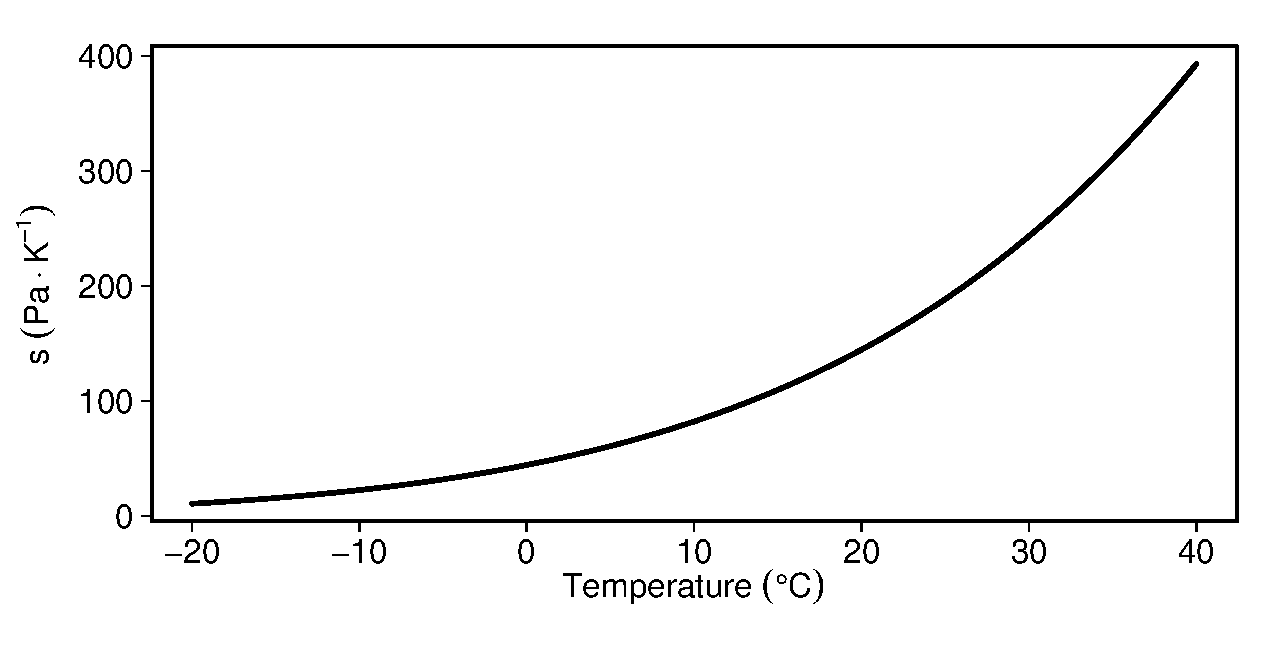
\includegraphics[width=\textwidth]{sat_slope.eps}
    \caption{The slope of the saturation vapor pressure temperature curve at temperatures from -20$^{\circ}$ to 40$^{\circ}$C.}
    \label{fig:sat}
\end{figure}

%% ------------------------------------------------------------------------ %%
%% eq:sat | Slope of saturation vapor pressure temperature curve, Pa/K
%% ------------------------------------------------------------------------ %%
\nomenclature{$s$}{Slope of saturation vapor pressure temperature curve, Pa$\cdot$K$^{-1}$}
\begin{equation}
\label{eq:sat}
	s = \frac{2.503\times 10^6\:\exp\left(\frac{17.27\: T_c}{T_c+237.3}\right) }
	              {\left(T_c+237.3\right)^2}
\end{equation}

\noindent where: \\
\indent $s$ = slope of saturation vapor pressure temperature curve, Pa$\cdot$K$^{-1}$ \\
\indent $T_c$ = ambient temperature, $^{\circ}$C \\

%% \\\\\\\\\\\\\\\\\\\\\\\\\\\\\\\\\\\\\\\\\\\\\\\\\\\\\\\\\\\\\\\\\\\\\\\\ %%
%% PART 2.09.3 -- LATENT HEAT OF VAPORIZATION, J/kg
%%///////////////////////////////////////////////////////////////////////// %%
\subsubsection{Latent heat of vaporization of water}
\label{sec:latent}
The enthalpy of vaporization (i.e., the latent heat of vaporization) of water has a dependency on temperature given by \parencite[Eq. 8]{henderson84}:

%% ------------------------------------------------------------------------ %%
%% fig:latent | Latent heat of vaporization, J/kg
%% ------------------------------------------------------------------------ %%
\begin{figure}[ht!]
    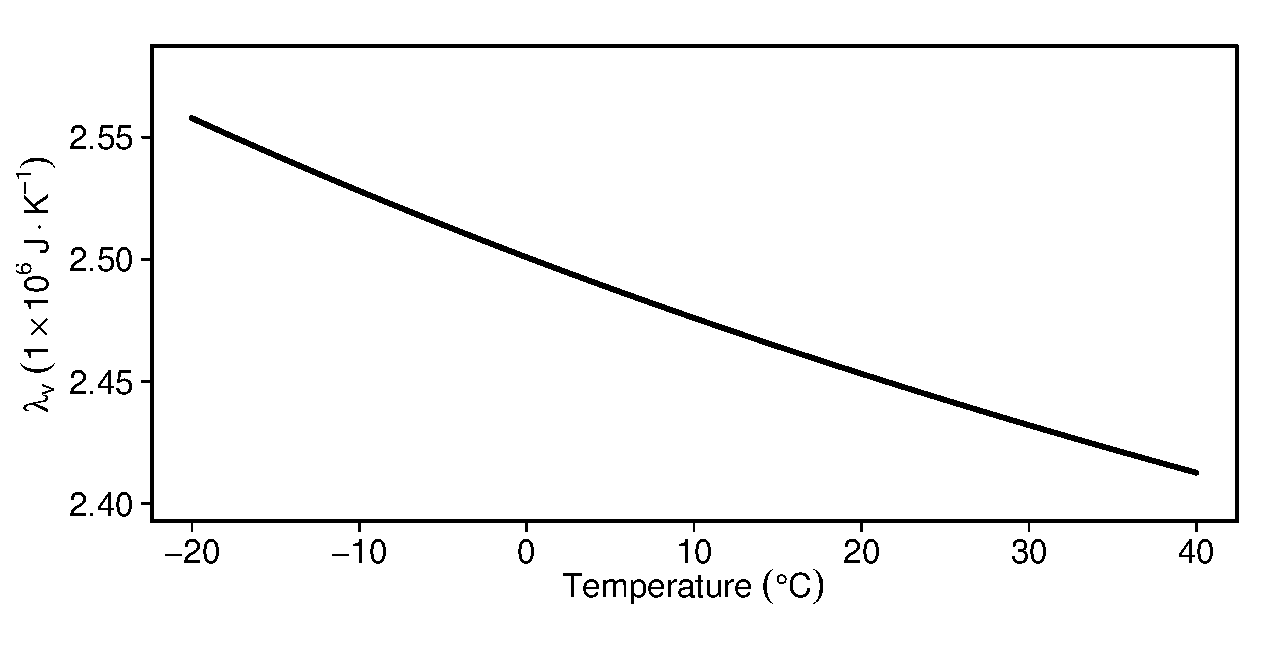
\includegraphics[width=\textwidth]{latent.eps}
    \caption{The latent heat of vaporization ($1\times 10^6$ J$\cdot$kg$^{-1}$) at temperatures from -20$^{\circ}$ to 40$^{\circ}$C.}
    \label{fig:latent}
\end{figure}

%% ------------------------------------------------------------------------ %%
%% eq:latent | Latent heat of vaporization, J/kg
%% ------------------------------------------------------------------------ %%
\nomenclature{$\lambda_v$}{Latent heat of vaporization of water, J$\cdot$kg$^{-1}$}
\begin{equation}
\label{eq:latent}
	\lambda_v = 1.91846\times 10^6\: \left(\frac{T_k}{T_k-33.91}\right)^2
\end{equation}

\noindent where: \\
\indent $\lambda_v$ = latent heat of vaporization of water, J$\cdot$kg$^{-1}$\\
\indent $T_k$ = ambient temperature, K\\

%% \\\\\\\\\\\\\\\\\\\\\\\\\\\\\\\\\\\\\\\\\\\\\\\\\\\\\\\\\\\\\\\\\\\\\\\\ %%
%% PART 2.09.4 -- DENSITY OF WATER, kg/m^3
%%///////////////////////////////////////////////////////////////////////// %%
\subsubsection{Density of water}
\label{sec:density}
The density of water depends on the temperature and (weakly) on the pressure \parencite{chen77}:

%% ------------------------------------------------------------------------ %%
%% fig:density | Density of water, kg/m^3
%% ------------------------------------------------------------------------ %%
\begin{figure}[ht!]
    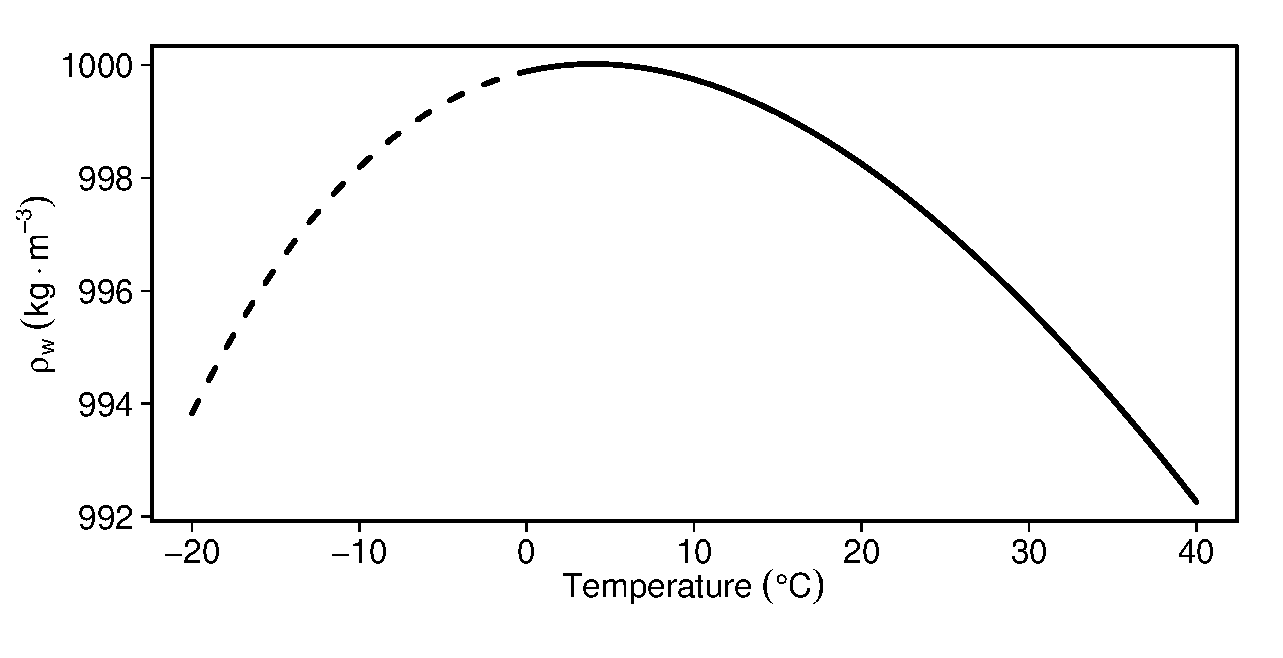
\includegraphics[width=\textwidth]{density.eps}
    \caption{The density of water at sea-level for temperatures from -20$^{\circ}$ to 40$^{\circ}$C (frozen water shown as dashed line).}
    \label{fig:density}
\end{figure}

%% ------------------------------------------------------------------------ %%
%% eq:density | Density of water, kg/m^3
%% ------------------------------------------------------------------------ %%
\nomenclature{$\rho_{w}$}{Density of water, kg$\cdot$m$^{-3}$}
\begin{equation}
\label{eq:density}
	\rho_w = 1000\: \rho_o \:\frac{K_o+C_A\: P_{bar}+C_B\: P_{bar}^2}
	               {K_o+C_A\: P_{bar} + C_B\: P_{bar}^2 - P_{bar}}
\end{equation}

\noindent where: \\
\indent $\rho_w$ = density of water, kg$\cdot$m$^{-3}$\\
\indent $\rho_o$ = density of water at 1 atm, g$\cdot$cm$^{-3}$\\
\indent $K_o$ = bulk modulus of water at 1 atm, bar\\
\indent $C_A$ = temperature-dependent coefficient, unitless\\
\indent $C_B$ = temperature-dependent coefficient, bar$^{-1}$\\
\indent $P_{bar}$ = atmospheric pressure, bar\\

\noindent The constant in Eq. \ref{eq:density} converts the units of density from g$\cdot$cm$^{-3}$ to kg$\cdot$m$^{-3}$. 
The following relationship may be used to convert between the units of atmospheric pressure: 1 bar $= 1\times 10^5$ Pa. 
The density of water at 1 atm may be calculated as \parencite{chen77, kell75}:

%% ------------------------------------------------------------------------ %%
%% eq:datm | Density of water at 1 atm, g/cm^3
%% ------------------------------------------------------------------------ %%
\nomenclature{$\rho_o$}{Density of water at 1 atmosphere, g$\cdot$cm$^{-3}$}
\begin{equation}
\label{eq:datm}
	\begin{split}
		\rho_o = & 0.99983952 + 6.78826\times 10^{-5}\: T_c \\
		          & -9.08659\times 10^{-6}\: T_c^2 + 1.02213\times 10^{-7}\: T_c^3\\
		          &-1.35439\times 10^{-9}\: T_c^4 + 1.47115\times 10^{-11}\: T_c^5\\
		          &-1.11663\times 10^{-13}\: T_c^6 + 5.04407\times 10^{-16}\: T_c^7\\
		          &-1.00659\times 10^{-18}\: T_c^8
	\end{split}
\end{equation}

\noindent where: \\
\indent $\rho_o$ = density of water at 1 atm, g$\cdot$cm$^{-3}$\\
\indent $T_c$ = ambient temperature, $^{\circ}$C\\

\noindent The bulk modulus of water at 1 atm may be calculated as \parencite{chen77, kell75}:

%% ------------------------------------------------------------------------ %%
%% eq:bulk | Bulk modulus of water at 1 atm, bar
%% ------------------------------------------------------------------------ %%
\nomenclature{$K_o$}{Bulk modulus of water at 1 atmosphere, bar}
\begin{equation}
\label{eq:bulk}
	\begin{split}
		K_o = & 19652.17 + 148.183\: T_c - 2.29995\: T_c^2 +0.01281\: T_c^3 \\
		          & -4.91564\times 10^{-5}\: T_c^4 +1.03553\times 10^{-7}\: T_c^5
	\end{split}
\end{equation}

\noindent where: \\
\indent $K_o$ = bulk modulus of water at 1 atm, bar\\
\indent $T_c$ = ambient temperature, $^{\circ}$C\\

\noindent The temperature-dependent coefficients, $C_A$ and $C_B$, are defined as \parencite{chen77}:

%% ------------------------------------------------------------------------ %%
%% eq:chena | Temperature-dependent coefficient, unitless
%% ------------------------------------------------------------------------ %%
\begin{equation}
\label{eq:chena}
	\begin{split}
		C_A = & 3.26138 +5.223\times 10^{-4}\: T_c +1.324\times 10^{-4}\: T_c^2\\
		       & -7.655\times 10^{-7}\: T_c^3 +8.584\times 10^{-10}\: T_c^4
	\end{split}
\end{equation}

%% ------------------------------------------------------------------------ %%
%% eq:chenb | Temperature-dependent coefficient, 1/bar
%% ------------------------------------------------------------------------ %%
\begin{equation}
\label{eq:chenb}
	\begin{split}
		C_B = & 7.2061\times 10^{-5} -5.8948\times 10^{-6}\: T_c +8.699\times 10^{-8}\: T_c^2 \\
		      & -1.01\times 10^{-9}\: T_c^3 +4.322\times 10^{-12}\: T_c^4
	\end{split}
\end{equation}

\noindent where: \\
\indent $C_A$ = temperature-dependent coefficient, unitless\\
\indent $C_B$ = temperature-dependent coefficient, bar$^{-1}$\\
\indent $T_c$ = ambient temperature, $^{\circ}$C\\

%% \\\\\\\\\\\\\\\\\\\\\\\\\\\\\\\\\\\\\\\\\\\\\\\\\\\\\\\\\\\\\\\\\\\\\\\\ %%
%% PART 2.09.5 -- PSYCHROMETRIC CONSTANT, Pa/K
%%///////////////////////////////////////////////////////////////////////// %%
\subsubsection{Psychrometric constant}
\label{sec:psychro}
The psychrometric constant depends on both the temperature and pressure. 
The pressure dependency is defined as \parencite[Eq. 8]{allen98}:

%% ------------------------------------------------------------------------ %%
%% fig:psychro | Psychrometric constant, Pa/K
%% ------------------------------------------------------------------------ %%
\begin{figure}[ht!]
    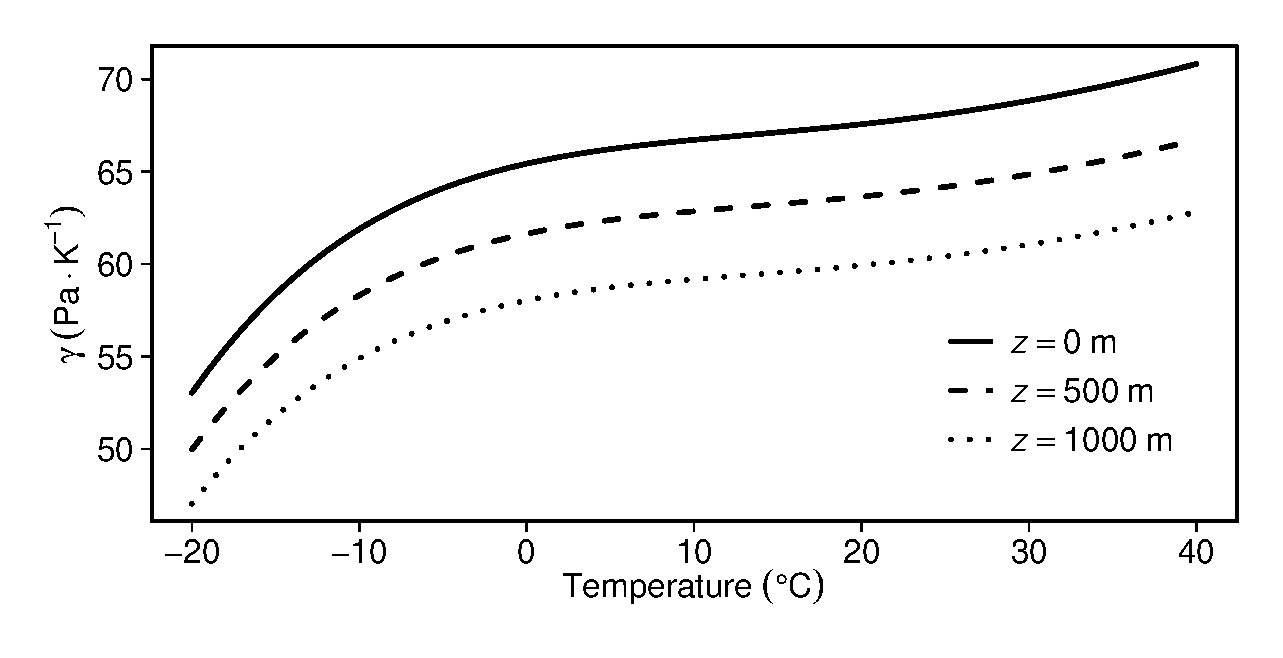
\includegraphics[width=\textwidth]{psychro.eps}
    \caption{The psychrometric constant at three elevations for temperatures from -20$^{\circ}$ to 40$^{\circ}$C.}
    \label{fig:psychro}
\end{figure}

%% ------------------------------------------------------------------------ %%
%% eq:psychro | Psychrometric constant, Pa/K
%% ------------------------------------------------------------------------ %%
\nomenclature{$\gamma$}{Psychrometric constant,  Pa$\cdot$K$^{-1}$}
\begin{equation}
\label{eq:psychro}
	\gamma = \frac{C_p\: M_a\: P_{a}}{M_v\: \lambda_v}
\end{equation}

\noindent where: \\
\indent $\gamma$ = psychrometric constant, Pa$\cdot$K$^{-1}$ \\
\indent $C_p$ = specific heat capacity of humid air, J$\cdot$kg$^{-1}\cdot$K$^{-1}$\\
\indent $M_a$ = molecular weight of dry air, kg$\cdot$mol$^{-1}$\\
\indent $M_v$ = molecular weight of water vapor, kg$\cdot$mol$^{-1}$\\
\indent $P_{a}$ = atmospheric pressure, Pa\\
\indent $\lambda_v$ = latent heat of vaporization of water, J$\cdot$kg$^{-1}$\\

\noindent Standard constants for $M_a$ and $M_v$ are given in Table \ref{tab:constants}. 
The latent heat of vaporization may either be assumed constant (e.g., $\lambda_v \approx 2.5\times 10^6$ J$\cdot$kg$^{-1}$) or it can be calculated (see \S \ref{sec:latent}). 
The specific heat capacity of humid air may either be assumed constant (e.g., $C_p \approx 1.013\times 10^3$ J$\cdot$kg$^{-1}\cdot$K$^{-1}$) or it can be calculated as a function of temperature \parencite[Eq. 47]{tsilingiris08}:

%% ------------------------------------------------------------------------ %%
%% fig:cp | Specific heat capacity of humid air, J/kg/K
%% ------------------------------------------------------------------------ %%
\begin{figure}[ht!]
    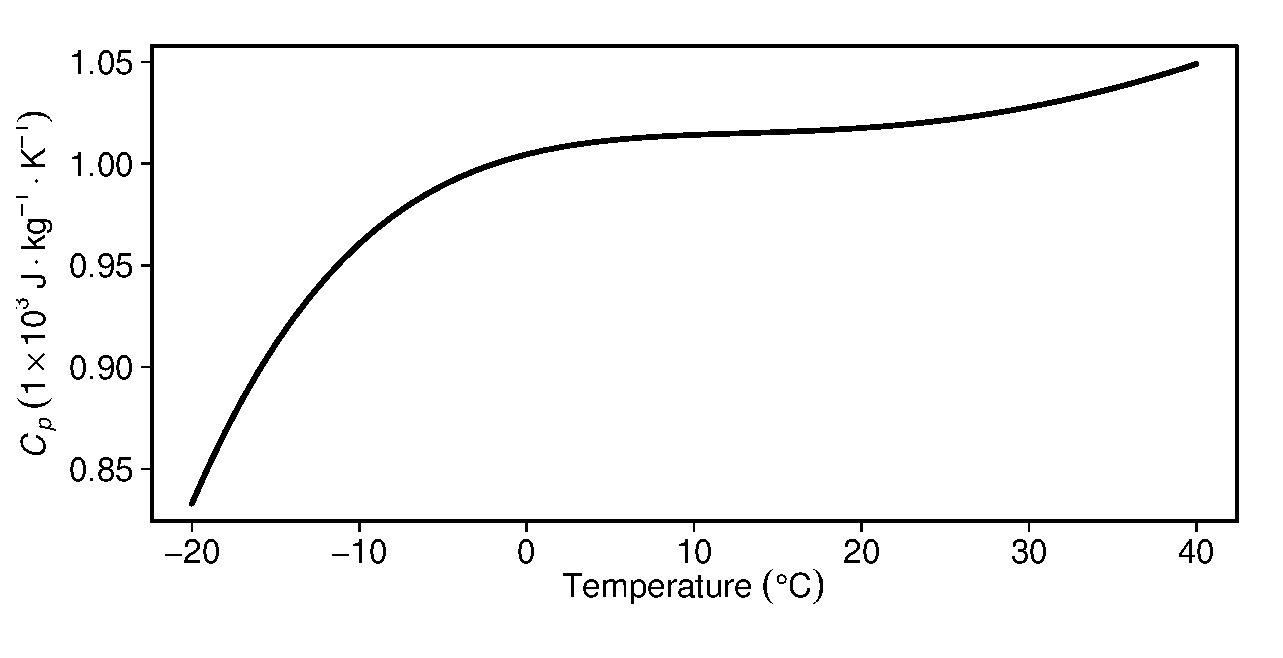
\includegraphics[width=\textwidth]{cp.eps}
    \caption{The specific heat capacity ($1\times 10^3$ J$\cdot$kg$^{-1}\cdot$K$^{-1}$) of humid air at temperatures from -20$^{\circ}$ to 40$^{\circ}$C.}
    \label{fig:cp}
\end{figure}

%% ------------------------------------------------------------------------ %%
%% eq:cp | Specific heat capacity of humid air, J/kg/K
%% ------------------------------------------------------------------------ %%
\nomenclature{$C_p$}{Specific heat capacity of humid air,   J$\cdot$kg$^{-1}\cdot$K$^{-1}$}\begin{equation}
\label{eq:cp}
	\begin{split}
		C_p = 1000\: ( &1.0045714270+2.050632750\times 10^{-3}\: T_c\\
		                              &-1.631537093\times 10^{-4}\: T_c^{2} 
		                                 +6.212300300\times 10^{-6}\: T_c^{3}\\
		                              &-8.830478888\times 10^{-8}\: T_c^{4} 
		                                 +5.071307038\times 10^{-10}\: T_c^{5} )
	\end{split}
\end{equation}

\noindent where: \\ 
\indent $C_p$ = specific heat capacity of humid air, J$\cdot$kg$^{-1}\cdot$K$^{-1}$\\
\indent $T_c$ = ambient temperature, $^{\circ}$C\\

%% \\\\\\\\\\\\\\\\\\\\\\\\\\\\\\\\\\\\\\\\\\\\\\\\\\\\\\\\\\\\\\\\\\\\\\\\ %%
%% PART 2.11 -- CONDENSATION, mm
%%///////////////////////////////////////////////////////////////////////// %%
\subsection{Condensation}
\label{sec:cond}
Condensation may be assumed equal to the water-equivalent of the nighttime net radiant energy (see \S \ref{sec:drnn}):

%% ------------------------------------------------------------------------ %%
%% eq:cond | Condensation, mm
%% ------------------------------------------------------------------------ %%
\nomenclature{$W_c$}{Daily condensation, mm}
\begin{equation}
\label{eq:cond}
	W_c = 1000\: E_{con}\: \lvert R_{Dnn} \rvert
\end{equation}

\noindent where: \\
\indent $W_c$ = daily nighttime condensation, mm\\
\indent $E_{con}$ = water to energy conversion factor, m$^{3}\cdot$J$^{-1}$\\
\indent $R_{Dnn}$ = daily nighttime total net radiation, J$\cdot$m$^{-2}$\\

%% \\\\\\\\\\\\\\\\\\\\\\\\\\\\\\\\\\\\\\\\\\\\\\\\\\\\\\\\\\\\\\\\\\\\\\\\ %%
%% PART 2.11 -- EQUILIBRIUM EVAPOTRANSPIRATION, mm/hr
%%///////////////////////////////////////////////////////////////////////// %%
\subsection{Equilibrium Evapotranspiration Rate}
\label{sec:eet}
The equilibrium evapotranspiration (EET) rate may be calculated as the water-equivalent of the net daytime radiation \parencite[Eq. 5]{prentice93}:

%% ------------------------------------------------------------------------ %%
%% eq:eet | Equilibrium evapotranspiration, mm/hr
%% ------------------------------------------------------------------------ %%
\nomenclature{$\text{EET}$}{Equilibrium evapotranspiration rate, mm$\cdot$hr$^{-1}$}
\begin{equation}
\label{eq:eet}
	\text{EET} = \left(1000\times 3600\right) \left(E_{con}\: R_n\right)
\end{equation}

\noindent where:\\
\indent EET = equilibrium evapotranspiration rate, mm$\cdot$hr$^{-1}$\\
\indent $E_{con}$ = water to energy conversion factor, m$^{3}\cdot$J$^{-1}$\\
\indent $R_n$ = net radiation flux, W$\cdot$m$^{-2}$ \\

\noindent Note that the two constants in Eq. \ref{eq:eet} convert the units from m$\cdot$s$^{-1}$ to mm$\cdot$hr$^{-1}$. 
There is no physical meaning for negative EET, and therefore EET should be set equal to zero when $R_n$ is negative. 

%% \\\\\\\\\\\\\\\\\\\\\\\\\\\\\\\\\\\\\\\\\\\\\\\\\\\\\\\\\\\\\\\\\\\\\\\\ %%
%% PART 2.12 -- DAILY EQUILIBRIUM EVAPOTRANSPIRATION, mm
%%///////////////////////////////////////////////////////////////////////// %%
\subsection{Daily Equilibrium Evapotranspiration}
\label{sec:deet}
The daily total equilibrium evapotranspiration can be calculated, as in \S \ref{sec:eet}, as the water-equivalent of the daily daytime net radiation (i.e., \S \ref{sec:drn}):

%% ------------------------------------------------------------------------ %%
%% eq:dayeet | Daily equilibrium evapotranspiration, mm
%% ------------------------------------------------------------------------ %%
\nomenclature{$\text{EET}_D$}{Daily equilibrium evapotranspiration, mm}
\begin{equation}
\label{eq:dayeet}
	\text{EET}_D = 1000\: \left(E_{con}\: R_{Dn}\right)
\end{equation}

\noindent where:\\
\indent EET$_D$ = daily equilibrium evapotranspiration, mm\\
\indent $E_{con}$ = water to energy conversion factor, m$^{3}\cdot$J$^{-1}$\\
\indent $R_{Dn}$ = daily total net radiation, J$\cdot$m$^{-2}$ \\

\noindent Note that the constant in Eq. \ref{eq:dayeet} converts the units from meters to millimeters.

%% \\\\\\\\\\\\\\\\\\\\\\\\\\\\\\\\\\\\\\\\\\\\\\\\\\\\\\\\\\\\\\\\\\\\\\\\ %%
%% PART 2.13 -- POTENTIAL EVAPOTRANSPIRATION RATE, mm/hr
%%///////////////////////////////////////////////////////////////////////// %%
\subsection{Potential Evapotranspiration Rate}
\label{sec:pet}
The potential evapotranspiration (PET) rate may exceed the equilibrium evapotranspiration rate (i.e., Eq. \ref{eq:eet}) by an entrainment factor \parencite{lhomme97, priestley72}:

%% ------------------------------------------------------------------------ %%
%% eq:pet | Potential evapotranspiration rate, mm/hr
%% ------------------------------------------------------------------------ %%
\nomenclature{$\text{PET}$}{Potential evapotranspiration rate, mm$\cdot$hr$^{-1}$}
\begin{equation}
\label{eq:pet}
	\text{PET} = \left(1000\times 3600\right) \left(1+w \right)\: \text{EET}
\end{equation}

\noindent where:\\
\indent PET = potential evapotranspiration rate, mm$\cdot$hr$^{-1}$\\
\indent $w$ = entrainment factor, unitless \\
\indent EET = equilibrium evapotranspiration rate, mm$\cdot$hr$^{-1}$\\

\noindent Note the two constants in Eq. \ref{eq:pet} convert the units from m$\cdot$s$^{-1}$ to mm$\cdot$hr$^{-1}$. Setting the entrainment factor, $w$, equal to zero sets PET equal to EET. 
A value of $w$ is given Table \ref{tab:constants}.

%% \\\\\\\\\\\\\\\\\\\\\\\\\\\\\\\\\\\\\\\\\\\\\\\\\\\\\\\\\\\\\\\\\\\\\\\\ %%
%% PART 2.14 -- DAILY POTENTIAL EVAPOTRANSPIRATION, mm
%%///////////////////////////////////////////////////////////////////////// %%
\subsection{Daily Potential Evapotranspiration}
\label{sec:dpet}
The daily total potential evapotranspiration is calculated by scaling the daily total equilibrium evapotranspiration (i.e., \S \ref{sec:deet}) by the entrainment factor, $w$:

%% ------------------------------------------------------------------------ %%
%% eq:daypet | Daily potential evapotranspiration, mm
%% ------------------------------------------------------------------------ %%
\nomenclature{$\text{PET}_D$}{Daily potential evapotranspiration, mm}
\begin{equation}
\label{eq:daypet}
	\text{PET}_D = \left(1+w \right) \: \text{EET}_D
\end{equation}

\noindent where:\\
\indent PET$_D$ = daily potential evapotranspiration, mm\\
\indent EET$_D$ = daily equilibrium evapotranspiration, mm\\
\indent $w$ = entrainment factor, unitless \\

%% \\\\\\\\\\\\\\\\\\\\\\\\\\\\\\\\\\\\\\\\\\\\\\\\\\\\\\\\\\\\\\\\\\\\\\\\ %%
%% PART 2.15 -- EVAPORATIVE DEMAND, mm
%% //////////////////////////////////////////////////////////////////////// %%
\subsection{Evaporative Demand}
\label{sec:dp}
The instantaneous evaporative demand is based on the potential evapotranspiration \parencite{federer82}:

%% ------------------------------------------------------------------------ %%
%% eq:dp | Evaporative demand rate, mm/hr
%% ------------------------------------------------------------------------ %%
\nomenclature{$D_p$}{Evaporative demand rate, mm$\cdot$hr$^{-1}$}
\begin{equation}
\label{eq:dp}
	D_p = \text{PET} = \left(1+w\right)\:\text{EET}
\end{equation}

\noindent where: \\
\indent $D_p$ = evaporative demand rate, mm$\cdot$hr$^{-1}$\\
\indent PET = potential evapotranspiration rate, mm$\cdot$hr$^{-1}$\\
\indent EET = equilibrium evapotranspiration rate, mm$\cdot$hr$^{-1}$\\

\noindent The evaporative demand, $D_p$ may also be expressed in terms of radiation fluxes. 
Based on Eq. \ref{eq:eet}, EET is related to the net radiation flux, which, based on Eq. \ref{eq:rn}, is the difference between net shortwave, $R_{ns}$ and net longwave, $R_{nl}$ radiation fluxes. 
The net shortwave radiation flux is related to the extraterrestrial radiation flux, $R_a$, through Eq. \ref{eq:rs} and Eq. \ref{eq:rns}, such that $D_p$ may be expressed as:

%% ------------------------------------------------------------------------ %%
%% eq:dpa | Evaporative demand rate (long expression), mm/hr
%% ------------------------------------------------------------------------ %%
\begin{equation}
\label{eq:dpa}
	D_p = \left(1000\times 3600\right) \left(1+w\right)\: E_{con}\:\left(
		\left(1-\beta\right)\:\tau\: R_a - R_{nl} \right)
\end{equation}

\noindent where:\\
\indent $w$ = entrainment factor, unitless \\
\indent $\beta$ = shortwave albedo, unitless \\
\indent $\tau$ = atmospheric transmittivity, unitless \\
\indent $R_{a}$ = extraterrestrial solar radiation flux, W$\cdot$m$^{-2}$ \\
\indent $R_{nl}$ = net longwave radiation, W$\cdot$m$^{-2}$ \\
\indent $E_{con}$ = water to energy conversion factor, m$^{3}\cdot$J$^{-1}$\\

\noindent Note the constants in Eq. \ref{eq:dpa} convert the units from m$\cdot$s$^{-1}$ to mm$\cdot$hr$^{-1}$. 
The total daily demand is based on the total daily PET (i.e., \S \ref{sec:dpet}) or the total daily daytime net radiation (i.e., \S \ref{sec:drn}):

%% ------------------------------------------------------------------------ %%
%% eq:daydp | Evaporative demand, mm
%% ------------------------------------------------------------------------ %%
\nomenclature{$D$}{Daily evaporative demand, mm}
\begin{equation}
\label{eq:daydp}
	D = \left(1+w\right)\:\text{EET}_D 
	  = 1000\:\left(1+w\right)\: E_{con}\: R_{Dn}
\end{equation}

\noindent where:\\
\indent $D$ = evaporative demand, mm\\
\indent EET$_D$ = daily equilibrium evapotranspiration, mm\\
\indent $R_{Dn}$ = daily daytime net radiation, J$\cdot$m$^{-2}$ \\

%% \\\\\\\\\\\\\\\\\\\\\\\\\\\\\\\\\\\\\\\\\\\\\\\\\\\\\\\\\\\\\\\\\\\\\\\\ %%
%% PART 2.16 -- ACTUAL EVAPOTRANSPIRATION RATE, mm/hr
%%///////////////////////////////////////////////////////////////////////// %%
\subsection{Actual Evapotranspiration Rate}
\label{sec:aet}
The actual evapotranspiration (AET) rate is based on the minimum of the supply and demand rates, as shown in Fig. \ref{fig:aet}, \parencite[Eq. 7]{federer82}:

%% ------------------------------------------------------------------------ %%
%% fig:aet | Actual evapotranspiration rate, mm/hr
%% ------------------------------------------------------------------------ %%
\begin{figure}[ht!]
    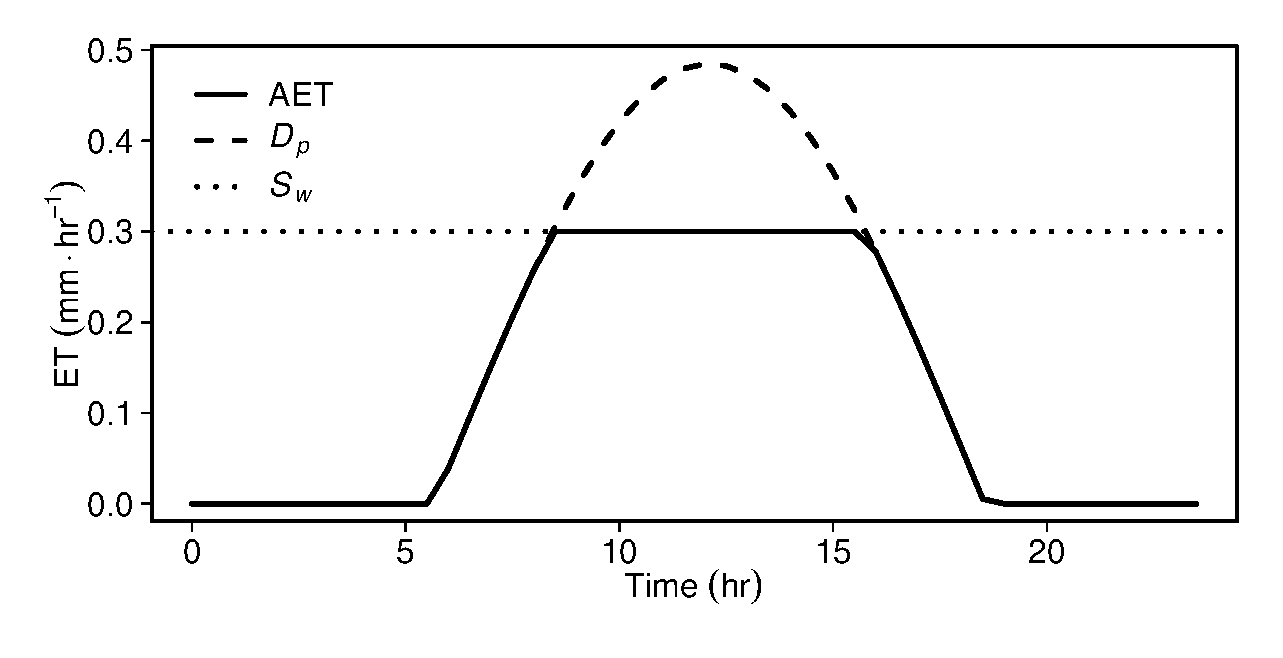
\includegraphics[width=\textwidth]{aet.eps}
    \caption{Example of the AET for a given $D_p$ when $S_w = 0.3$ mm$\cdot$hr$^{-1}$.}
    \label{fig:aet}
\end{figure}

%% ------------------------------------------------------------------------ %%
%% eq:aet | Actual evapotranspiration rate, mm/hr
%% ------------------------------------------------------------------------ %%
\nomenclature{$\text{AET}$}{Actual evapotranspiration rate, mm$\cdot$hr$^{-1}$}
\begin{equation}
\label{eq:aet}
	\text{AET} = \min\left(S_w\text{, }D_p\right)
\end{equation}

\noindent where:\\
\indent AET = actual evapotranspiration rate, mm$\cdot$hr$^{-1}$\\
\indent $S_w$ = evaporative supply rate, mm$\cdot$hr$^{-1}$\\
\indent $D_p$ = evaporative demand rate, mm$\cdot$hr$^{-1}$\\

\noindent Note that the minimization is based on the instantaneous rates and not the daily totals!

%% \\\\\\\\\\\\\\\\\\\\\\\\\\\\\\\\\\\\\\\\\\\\\\\\\\\\\\\\\\\\\\\\\\\\\\\\ %%
%% PART 2.17 -- DAILY ACTUAL EVAPOTRANSPIRATION, mm
%%///////////////////////////////////////////////////////////////////////// %%
\subsection{Daily Actual Evapotranspiration}
\label{sec:daet}
The daily actual evapotranspiration can be analytically solved similar to the methods used for $R_{Da}$ (i.e., \S \ref{sec:dra}) and $R_{Dn}$ (i.e., \S \ref{sec:drn}). 
Analogous to the sunset hour angle, $H_s$, and net radiation flux cross-over hour angle, $H_n$, a new hour angle must be defined relating to the point when $D_p = S_w$. 
This intersection hour angle, $H_i$, is found by setting the equation for $D_p$ equal to $S_w$. 
Using the variable substitutions defined in \S \ref{sec:drn} and letting $r_x = 1000\cdot 3600\cdot\left(1+w\right)\cdot E_{con}$, $D_p$ may be expressed as:

%% ------------------------------------------------------------------------ %%
%% eq:dpb | Evaporative demand rate (substitue expression), mm/hr
%% ------------------------------------------------------------------------ %%
\begin{equation}
\label{eq:dpb}
	D_p = r_x\:\left(
		 r_w\:\left(r_u+r_v\:\cos H\right)- R_{nl} 
		 \right)
\end{equation}

\noindent Setting Eq. \ref{eq:dpb} equal to $S_w$ and solving for the hour angle:

%% ------------------------------------------------------------------------ %%
%% eq:hi | Intersecting hour angle, radians
%% ------------------------------------------------------------------------ %%
\nomenclature{$H_i$}{Supply and demand intersecting hour angle, radians}
\begin{equation}
\label{eq:hi}
	H_i = \arccos \left( \frac{S_w}{r_x\: r_w\: r_v}
	                   + \frac{R_{nl}}{r_w\: r_v}
	                   - \frac{r_u}{r_v} \right)
\end{equation}

\noindent where:\\
\indent $H_i$ = supply and demand intersecting hour angle, radians\\
\indent $S_w$ = evaporative supply rate, mm$\cdot$hr$^{-1}$\\
\indent $r_u = \sin\delta\cdot\sin\phi$, unitless \\
\indent $r_v = \cos\delta\cdot\cos\phi$, unitless \\
\indent $r_w = \left(1-\beta\right)\cdot\tau\cdot G_{sc}\cdot d_r$, W$\cdot$m$^{-2}$\\
\indent $r_x = 1000\cdot 3600\cdot\left(1+w\right)\cdot E_{con}$, $($mm$\cdot$hr$^{-1})\cdot ($W$\cdot$m$^{-2})^{-1}$\\

\noindent Special care needs to be made when $\cos\left( H_i\right) \geq 1$ (i.e., supply rate exceeds demand, $H_i = 0$) and when $\cos\left( H_i\right) \leq -1$ (i.e., supply rate limits demand everywhere, $H_i = \pi$). Note that as $S_w$ approaches zero, $H_i$ approaches $H_n$ (i.e., Eq. \ref{eq:hns}).

The half-day integral of actual evapotranspiration consists of two parts: the $S_w$ curve from solar noon, $H_o$, to the intersection hour angle, $H_i$, and the $D_p$ curve from $H_i$ to the net radiation cross-over angle, $H_n$:

%% ------------------------------------------------------------------------ %%
%% eq:iaet | Integrals for AET
%% ------------------------------------------------------------------------ %%
\begin{equation}
\label{eq:iaet}
	\int_{H_o}^{H_n} \text{AET} = \int_{H_o}^{H_i} S_w + \int_{H_i}^{H_n} D_p
\end{equation}

Integrating Eq. \ref{eq:iaet} and using the variable substitution as in Eq. \ref{eq:hi}:

%% ------------------------------------------------------------------------ %%
%% eq:intaet | Integrating AET
%% ------------------------------------------------------------------------ %%
\begin{equation}
\label{eq:intaet}
	\begin{split}
		\int_{H_o}^{H_n} \text{AET} = & S_w\: H_i + r_x\: r_w\: r_v \: \left(\sin H_n - \sin H_i\right) \\
		& + r_x\:\left(r_w\: r_u - R_{nl}\right)\:\left(H_n-H_i\right)
	\end{split}
\end{equation}

\noindent Note that when $S_w$ exceeds $D_p$ (i.e., $H_i = 0$), Eq. \ref{eq:intaet} becomes equivalent to Eq. \ref{eq:daydp}.

The daily actual evapotranspiration, AET$_D$, is found by doubling the quantity in Eq. \ref{eq:intaet} and converting the units integrated over from radians to hours:

%% ------------------------------------------------------------------------ %%
%% eq:dayaet | Daily AET, mm
%% ------------------------------------------------------------------------ %%
\nomenclature{$\text{AET}_D$}{Daily actual evapotranspiration, mm}
\begin{equation}
\label{eq:dayaet}
	\begin{split}
		\text{AET}_D = & \frac{24}{\pi}\: ( S_w\: H_i \\
		& + r_x\: r_w\: r_v \: \left(\sin H_n - \sin H_i\right) \\
		& + \left(r_x\: r_w\: r_u - r_x\: R_{nl}\right)\left(
		    H_n-H_i\right))
	\end{split}
\end{equation}

\noindent where:\\
\indent AET$_D$ = daily actual evapotranspiration, mm\\
\indent $S_w$ = evaporative supply rate, mm$\cdot$hr$^{-1}$\\
\indent $H_i$ = supply and demand intersecting hour angle, radians\\
\indent $H_n$ = net radiation flux cross-over hour angle, radians\\
\indent $r_u = \sin\delta\cdot\sin\phi$, unitless \\
\indent $r_v = \cos\delta\cdot\cos\phi$, unitless \\
\indent $r_w = \left(1-\beta\right)\cdot\tau\cdot G_{sc}\cdot d_r$, W$\cdot$m$^{-2}$\\
\indent $r_x = 1000\cdot 3600\cdot\left(1+w\right)\cdot E_{con}$, $($mm$\cdot$hr$^{-1})\cdot ($W$\cdot$m$^{-2})^{-1}$\\

%% \\\\\\\\\\\\\\\\\\\\\\\\\\\\\\\\\\\\\\\\\\\\\\\\\\\\\\\\\\\\\\\\\\\\\\\\ %%
%% PART 2.18 -- DAILY SOIL MOISTURE, mm
%%///////////////////////////////////////////////////////////////////////// %%
\subsection{Daily Soil Moisture}
\label{sec:dw}
The daily soil moisture, $W_n$, is calculated by adding the daily precipitation, $P_n$, and daily condensation, $W_c$ (see \S \ref{sec:cond}), to yesterday's soil moisture and subtracting the daily actual evapotranspiration, AET$_D$ (see \S \ref{sec:daet}) \parencite{cramer88}:

%% ------------------------------------------------------------------------ %%
%% eq:dw | Daily soil moisture, mm
%% ------------------------------------------------------------------------ %%
\nomenclature{$W_n$}{Daily soil moisture, mm}
\begin{equation}
\label{eq:dw}
	W_n = W_{n-1} + P_n + W_c - \text{AET}_D
\end{equation}

\noindent where: \\
\indent $W_n$ = daily soil moisture, mm\\
\indent $P_n$ = daily precipitation, mm\\
\indent $W_c$ = daily nighttime condensation, mm\\
\indent AET$_D$ = daily actual evapotranspiration, mm\\

\noindent Note that daily soil moisture may exceed the soil moisture capacity, $W_m$. 
In such a case, the excess water is considered runoff and may be calculated as the maximum of zero or the difference between daily soil moisture and the moisture capacity:

%% ------------------------------------------------------------------------ %%
%% eq:ro | Daily runoff, mm
%% ------------------------------------------------------------------------ %%
\nomenclature{$RO$}{Daily runoff, mm}
\begin{equation}
\label{eq:ro}
	RO = \max\left(0\text{, }W_n-W_m\right)
\end{equation}

\noindent where: \\
\indent $RO$ = daily runoff, mm\\
\indent $W_n$ = daily soil moisture, mm\\
\indent $W_m$ = soil moisture capacity, mm\\

\noindent Following the runoff calculation, daily soil moisture must be set within the physical limits (i.e., $0\leq W_n\leq W_m$) before calculating tomorrow's evaporative supply and soil moisture quantities:

%% ------------------------------------------------------------------------ %%
%% eq:wn | Setting daily soil moisture within physical limits
%% ------------------------------------------------------------------------ %%
\begin{equation}
\label{eq:wn}
	W_n = 
	\begin{cases}
		W_m, & \text{if } W_n \geq W_m\\
		0, & \text{if } W_n \leq 0
	\end{cases}
\end{equation}

%% \\\\\\\\\\\\\\\\\\\\\\\\\\\\\\\\\\\\\\\\\\\\\\\\\\\\\\\\\\\\\\\\\\\\\\\\ %%
%% PART 2.19 -- CRAMER-PRENTICE MOISTURE INDEX, alpha
%%///////////////////////////////////////////////////////////////////////// %%
\subsection{Cramer-Prentice Moisture Index}
\label{sec:alpha}
The Cramer-Prentice bioclimatic moisture index, $\alpha$, is calculated as \parencite[as described in][]{sykes96, gallego-sala10}:

%% ---------------------------------------------------------------%%
%% eq:alpha | Cramer-Prentice moisture index, unitless
%% ---------------------------------------------------------------%%
\nomenclature{$\alpha$}{Monthly Cramer-Prentice moisture index, unitless}
\begin{equation}
\label{eq:alpha}
	\alpha = \frac{\sum_{i=1}^{N_m} \text{AET}_{Di}}
	              {\sum_{i=1}^{N_m} \text{EET}_{Di}}
\end{equation}

\noindent where:\\
\indent $i$ = day of the month (i.e., 1--31) \\
\indent $N_m$ = number of days in a month \\
\indent $\alpha$ = monthly Cramer-Prentice moisture index, unitless \\
\indent AET$_D$ = daily actual evapotranspiration, mm\\
\indent EET$_D$ = daily potential evapotranspiration, mm\\

Due to the fact that AET follows PET during the course of the day and given the definition of daily PET (see \S \ref{sec:dpet}), the value of $\alpha$ is expected to range between 0 and $1+w$ (e.g., 1.26, when $w=0.26$). 

%% \\\\\\\\\\\\\\\\\\\\\\\\\\\\\\\\\\\\\\\\\\\\\\\\\\\\\\\\\\\\\\\\\\\\\\\\ %%
%% PART 2.20 -- CLIMATIC WATER DEFICIT, mm
%%///////////////////////////////////////////////////////////////////////// %%
\subsection{Climatic Water Deficit}
\label{sec:cwd}
The climatic water deficit is a measure of the difference between actual and potential evapotranspiration \parencite{stephenson98}:

%% ---------------------------------------------------------------%%
%% eq:cwd | Climatic water deficit, mm
%% ---------------------------------------------------------------%%
\nomenclature{$\Delta\text{E}$}{Monthly climatic water deficit, mm}
\begin{equation}
\label{eq:cwd}
	\Delta\text{E} = \sum_{i=1}^{N_m} \left(
	                 \text{PET}_{Di} - \text{AET}_{Di} \right)
\end{equation}

\noindent where:\\
\indent $i$ = day of the month (i.e., 1--31) \\
\indent $N_m$ = number of days in a month \\
\indent $\Delta$E = monthly climatic water deficit, mm \\
\indent AET$_D$ = daily actual evapotranspiration, mm\\
\indent PET$_D$ = daily potential evapotranspiration, mm\\
